\documentclass{article}


% if you need to pass options to natbib, use, e.g.:
%     \PassOptionsToPackage{numbers, compress}{natbib}
% before loading neurips_2024


% ready for submission
%\usepackage{neurips_2024}


% to compile a preprint version, e.g., for submission to arXiv, add add the
% [preprint] option:
\usepackage[preprint]{neurips_2024}


% to compile a camera-ready version, add the [final] option, e.g.:
%     \usepackage[final]{neurips_2024}


% to avoid loading the natbib package, add option nonatbib:
%    \usepackage[nonatbib]{neurips_2024}


\usepackage[utf8]{inputenc} % allow utf-8 input
\usepackage[T1]{fontenc}    % use 8-bit T1 fonts
\usepackage{hyperref}       % hyperlinks
\usepackage{url}            % simple URL typesetting
\usepackage{booktabs}       % professional-quality tables
\usepackage{amsfonts}       % blackboard math symbols
\usepackage{nicefrac}       % compact symbols for 1/2, etc.
\usepackage{microtype}      % microtypography
\usepackage{xcolor}         % colors
\usepackage{wrapfig}
\usepackage{multicol}
\usepackage{epsfig}
\usepackage{subfig}
\usepackage{svg}
\usepackage{amsmath}
\usepackage{wrapfig}


\title{Creating Synthetic Genomes using Diffusion Models}


% The \author macro works with any number of authors. There are two commands
% used to separate the names and addresses of multiple authors: \And and \AND.
%
% Using \And between authors leaves it to LaTeX to determine where to break the
% lines. Using \AND forces a line break at that point. So, if LaTeX puts 3 of 4
% authors names on the first line, and the last on the second line, try using
% \AND instead of \And before the third author name.


\author{%
  Philip Kenneweg\\
  AG Machine Learning\\
  University of Bielefeld\\
  \texttt{pkenneweg@*} \\
  \And
  Raghuram Dandinasivara\\
  AG Genome Data Science\\
  University of Bielefeld\\
  \texttt{rdandinasivara@*} \\
  \And
  Alexander Schönhut\\
  AG Genome Data Science\\
  University of Bielefeld\\
  \texttt{aschoen@*}\\
  \And
  Barbara Hammer\\
  AG Machine Learning\\
  University of Bielefeld\\
  \texttt{bhammer@*}\\
  *@techfak.uni-bielefeld.de
  % examples of more authors
  % \And
  % Coauthor \\
  % Affiliation \\
  % Address \\
  % \texttt{email} \\
  % \AND
  % Coauthor \\
  % Affiliation \\
  % Address \\
  % \texttt{email} \\
  % \And
  % Coauthor \\
  % Affiliation \\
  % Address \\
  % \texttt{email} \\
  % \And
  % Coauthor \\
  % Affiliation \\
  % Address \\
  % \texttt{email} \\
}


\begin{document}


\maketitle


\begin{abstract}

In this paper, we introduce the first diffusion model designed to generate complete synthetic human genomes. These genomes closely mimic real human genomes and serve as a nearly perfect substitute for genuine ones in disease classification tasks. This innovation addresses a significant challenge in current research: real human genomes are highly sensitive private data and cannot be widely distributed due to privacy concerns. By using synthetic genomes, researchers can train AI models and identify correlations without stringent data privacy measures. Additionally, training diffusion models allows the inclusion of unlabeled data, reducing the reliance on large labeled datasets.

%In this paper we present the first diffusion model capable of generating a complete synthetic human genome. These synthetic genome are realistic enough to be an almost perfect substitute for real human genomes in disease classification tasks. Thus we are able to solve a common problem in current research, real human genomes are very sensitive private data and can not be distributed widely. Synthetic human genomes do no longer have privacy concerns and can thus be used to train AI models, find correlations and much more without the need for rigorous data privacy measures. Another benefit of this approach is that unlabeled data can be incorporated in training diffusion models, thus reducing the need for large amounts of accurate labels.
%Generating realistic human genomes is a 

 %In this paper we present the first full human genome diffusion model. It is capable of generating a complete synthetic human genome. This can be used to train classification models, which generalize on unseen data. The benefits of this technology are the elimination of privacy concerns, as well as the usage of modern unsupervised deep learning technology to better generalize to unseen data. We are confident that this first step enables a wide variety of future applications.
\end{abstract}


\section{Introduction}

The field of deep learning has enabled various breakthrough technologies in the biotech sector \citep{alphafold, wong2024discovery, cheng2023accurate}. While these technologies constitute major advancements, they investigated inputs in the form of small sections of available data due to computational constraints. In this work we take the first steps towards processing the whole human genome at once using modern deep learning techniques, while keeping the required compute to a minimum.

A major problem when analyzing human genomes is the size of the data as well as the high amount of complexity inherent in the data and unclear interaction pathways between different genomes. 

In \citet{yelmen2021creating} they use GAN networks to generate small sections of human genomes and use a variety of metrics like linkage disequilibirum and nearest neighbour adversarial accuracy to measure the quality of their creates genomes.

We postulate that by compressing the human genome using prior biological knowledge, as well as using the latest deep learning techniques,
%consisting of unsupervised learning on large scale data, 
we can solve the common problem of sharing highly sensitive data by replacing the real data with high quality synthetic data. 


\section{Related Work}
\label{sec:related_work}


\subsection{Unsupervised Learning on Genetic Data}

A popular paradigm in recent successful deep learning schemes, is pre-training large models on unlabeled data to make use of large amounts of training data, without needing tedious or sometimes impossible human provided labels.

The transformer model \citep{vaswani2017attention} popularized this approach on the natural language domain by combining it with architectures capable of learning arbitrary relations in data. 

The same approach is possible for the genetics domain and will enable many use cases previously thought impossible, similar to the language domain.

\subsection{Working with Long Sequences}

A common problem when working with genetic data is the size of the data and the long range interactions which have to be considered.

HyenaDNA \citep{nguyen2023hyenadna} is a powerful state of the art transformer based architecture which is able to process up to a million tokens at once using an adapted form of attention. But even with this latest technology it fails to be able to process whole human genomes which are about 3 billion base pairs long.

Research in deep learning has investigated projecting data into a shared embedding space in which long sequences can be greatly compressed. The most widely known use case for this is the Vision Transformer \citep{dosovitskiy2021an} which works directly with images, even though transformers typically can not process sequences of these sizes due to computational limitations. They achieve this feat by compressing regions, they call patches of an image into a single embedding. This shared projection is typically done by a small MLP or CNN which is the same for each image region. 

Other works, especially in the diffusion domain, for example Stable Diffusion by \cite{rombach2021highresolution} have also adopted the paradigm of no longer working directly on the data but rather on a compressed version of it. This is typically called working in the embedding space and we take great inspiration from this principle.

\subsection{Diffusion Models}
In this section we will give a rough outline of the diffusion process used. For a more detailed look at diffusion processes we recommend the works by \cite{ddpm, ddim}
\subsubsection{Training}
Diffusion Models are a relatively new sub-field in generative AI which add Gaussian noise $\epsilon = N(\mu,\sigma)$ with variance $\sigma = 1$ and mean $\mu = 0$ to data $x \in D$ to generate noised data $x_n$ according to some noise schedule in $t \in (0,T)$ steps.

First we define some helpful variables:
\begin{equation}
   \alpha(t) = 1-\beta(t)  ;
   \overline{\alpha}(t) = \prod_{s=1}^t \alpha_s ;
   \Tilde{\beta}(t) = \frac{1-\overline{\alpha}(t-1)}{1-\overline{\alpha}(t)}\beta(t)
\end{equation}

where $\beta_t$ represents the variances of the forward process, in practice it is a pre-determined scalar schedule increasing linearly from $\beta(1) = 10^{-4}$ to $\beta(T) = 0.02$, see \cite{ddpm}.

\begin{equation}
    x_n(t) = \sqrt{\overline{\alpha}(t)} \cdot \epsilon + \sqrt{1-\overline{\alpha}(t)}\cdot x
\end{equation}

The process is designed for a data distribution $D$ with mean $\sigma = 1$ and variance $\mu = 0$, which are easy pre-processing steps. 


The recovery task is given the noised image and the noise schedule $t,x_n$ to predict the previously added noise $\epsilon$ we call the predicted noise $\epsilon_p$. This is typically realized by an artificial neural network $E$. 

\begin{equation}
     \epsilon_{p} = E(t,x_n(t))
     \label{eq:nn}
\end{equation}

To recover the original data $x$ in a single step the predicted $x_p$ can be computed according to:
\begin{equation}
    x_p(t,x) = \frac{x_n(t) - (1-\sqrt{\overline{\alpha}(t)}) \cdot \epsilon_p}{\sqrt{\overline{\alpha}(t)}}
    \label{eq:denoise}
\end{equation}

The loss function $L(x)$ of our neural network is simply:

\begin{equation}
    L(x) = ||\epsilon,\epsilon_p(x)||
\end{equation}

where $||\cdot,\cdot||$ is some distance norm, in our case we use the L2 norm also called mean squared error. The loss is not based on the recovered data $x_p$ as the predicted noise $\epsilon_p$ contains the same information but with less intermediate steps.
%Typically t is chosen as an integer value between 1 and 1000 and then scaled into the range $(0,1)$ by dividing with the maximum step e.g. 1000. 
During training $t$ is drawn from a uniform random distribution for each input sample.

\subsubsection{Data Generation}
Generating new data is done analogously to recovering the original data. Starting from complete noise $x_{n,T} = N(0,I)$, the newly generated data-point is recovered by iteratively refining the prediction of new noised $x_p$ according to Eq \ref{eq:denoise} but each step $t$ new noise is added to remain in the same distribution as the original $x_n$. 




\begin{equation}
    x_{n,t-1} = \frac{1}{\sqrt{\alpha(t)}} \cdot (x_{t} - \frac{1-\alpha(t)}{\sqrt{1-\overline{\alpha}(t)}} \epsilon_p(x_{n,t},t)) + \sqrt{\Tilde{\beta}(t)}  N(0,I) %t_{k-1} \cdot \epsilon + (1-t_{k}) \cdot x_{p,k}(t_{k},x_{k})
    \label{eq:generation}
\end{equation}

This process is called DDPM \citep{ddpm} and has been highly successful in generating realistic artificial images and other data. 
\bigbreak
Furthermore, more information can be incorporated by presenting so called conditioning information $y$ to the neural network, changing Equation \ref{eq:nn} to:

\begin{equation}
    \epsilon_{p} = E(t,x_n(t),y)
\end{equation}

typically $y$ is an input vector containing additional information about the data sample $x$. For example, in the image case this could be the caption of the image, or whether or not a certain class is present in the image.

% The data generation process can be sped up by not taking every single step but only a subset in intervalls $dt$, this is accomplished by following DDIM \citep{ddim}, changing Equation \ref{eq:generation} to:
% \begin{equation}
%     x_{n,t-dt} = \sqrt{\overline{\alpha}(t-dt)} * x_p(t,x) + \sqrt{1-\overline{\alpha}(t-dt)} * \epsilon_p
%     \label{eq:ddim}
% \end{equation}

% \subsection{Classifier Free Guidance}
% In the image generation domain it was found that classifier free guidance \cite{} is crucial to obtain high quality images that are aligned with the given conditioning.

% We obtain both the conditioned $\epsilon_{p,c} = E(t,x_n(t),y)$ and the unconditioned output $\epsilon_{p,u} = E(t,x_n(t))$  of the model. Following, they are combined to guide the generation process by changing Equation \ref{eq:nn} to:

% \begin{equation}
%     \epsilon_p = (1+\lambda) \epsilon_{p,c} - \lambda \epsilon_{p,u}
% \end{equation}

% % \begin{equation}
% %     x_p(t,x) = \frac{x_n(t) - t \cdot ((1+\lambda) \cdot \epsilon_{p,c} - \lambda \cdot \epsilon_{p,u})}{1-t}
% % \end{equation}

% By modifying guidance parameter $\lambda \in (0,\infty)$ we can choose how strong the conditioning guides the generation process. $\lambda = 0$ results in the normal conditioned generation process, while $\lambda = \infty$ only produces features which are important to the conditioning. Typically values for image networks are in the range of $(0.5,3)$.

\section{Methods}
\label{sec:methods}


To generate synthetic data and thereby enable sharing of genetic data without privacy concerns we train a diffusion model on real data to produce an arbitrary amount of synthetic data.
\subsection{Data}

Although in this work we establish a model that is generic with respect to the kind of SNPs of a human genome it can predict, we focus on the occurrence/prevalence of ALS as a phenotype in the following. The reasons for this are the availability of the excellent, sufficiently large amounts of data that were raised in the frame of Project MinE \citet{project2018project}. Most importantly, we emphasize ALS, based on the aforementioned large missing heritability. For analogous reasons, also the earlier related studies \citep{auer2012imputation, dolzhenko2017detection} rely on data raised in the frame of Project MinE. 


The data on which we are working on has 18.279 genes sequenced for 10.405 humans. Each of these genes is a sequence of between 5-100 different SNPs.


\subsection{Data Pre-processing}
First we take a closer look at the available data and how it can be compressed to facilitate deep learning on it.% For this compression we closesly follow already established methods \citep{capsulenet}.

A human genome consists of 3 billion base pairs. Analyzing the whole genome for each use case is generally not possible due to its length.
A common alternative in biotech is analyzing the parts of the human genome which change between individual humans. This is done using single nucleotide polymorphisms (SNP). Data in this form is available from \cite{project2018project}.

To further compress this data and make it usable we follow the protocol from \citet{capsulenet}, where these SNPs are individually compressed using Principle Component Analysis (PCA) of varying lengths, up to a maximum of 8 dimensions. This further reduces the dimensionality while incurring minimal compression loss ($<1\%$). A rough outline of this process can be seen in Figure \ref{fig:pca}

\begin{wrapfigure}{r}{0.5\textwidth}
    \centering
    
    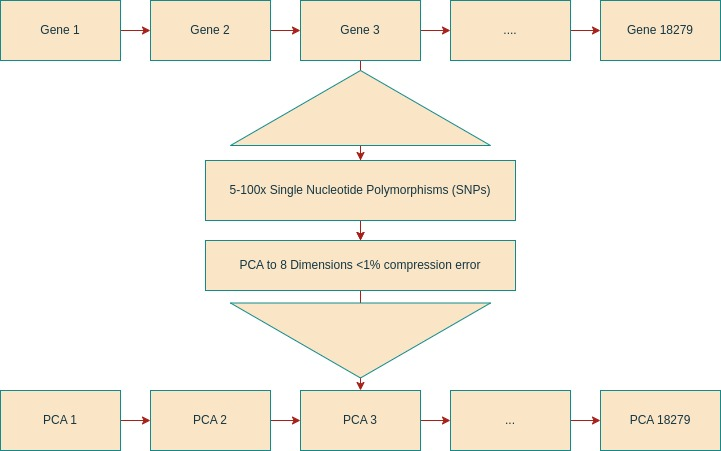
\includegraphics[width = 0.48\textwidth]{figures/preprocess.jpg}
    \caption{Pre-processing pipeline}
    \label{fig:pca}
\end{wrapfigure}

For further pre-processing we zero-pad all PCAs to be of length $8$ to produce a vector of $x \in \mathbb{R}^{18279\times8}$ as a representation of our data. We further pad this with zeroes to be $x \in \mathbb{R}^{18432\times8}$ for efficiency gains on modern architectures ($18432$ is divisible by $2^{11}$). We found that all of this zero-padding, while necessary, results in samples leaving the typically input distribution during the diffusion generation process. To remedy this we set the loss $L(x)$ at all zero padded position to zero, as well as modify the diffusion process by clamping all zero padded positions of $x_p$ to zero. Note that the zero padding is the same for all inputs, so this operation is easy and efficient to apply.


%See Methods for exact descriptions of the data. Note that available data is hard to come by in a real life setting. We focus on data produced by https://www.projectmine.com/ which is high quality whole human genome analysis with a large amount of SNPs analyzed.

\begin{wrapfigure}{r}{0.5\textwidth}
    \centering
    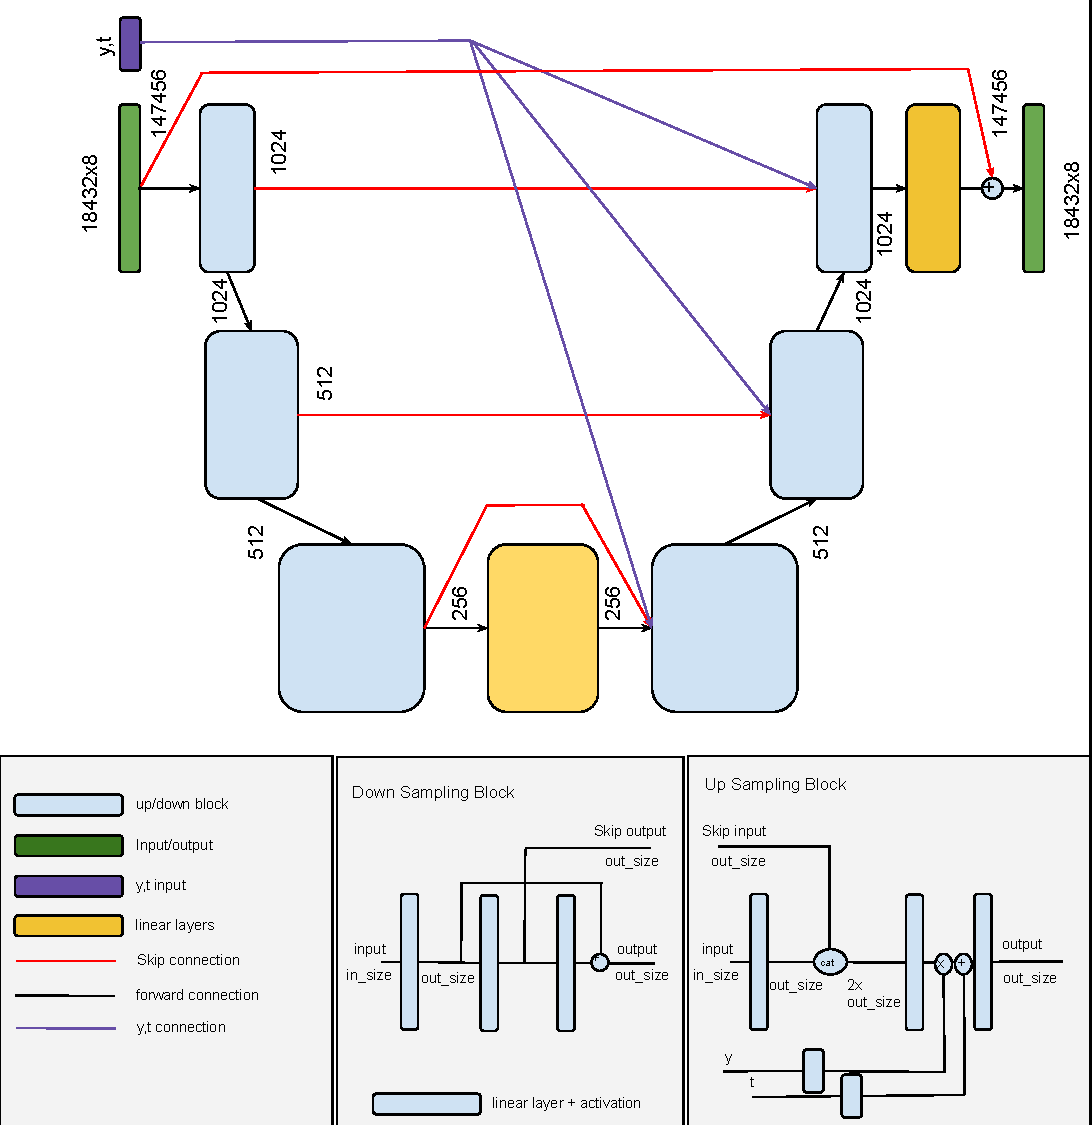
\includegraphics[width = 0.48\textwidth]{figures/UnetMLP.pdf}
   % \includefigure[width = 0.48\textwidth]{figures/UnetMLP.pdf}
    \caption{A structural overview of the architecture of the MLP diffusion model.}
    \label{fig:unet}
\end{wrapfigure}

\subsection{Model Architecture}
We base our Diffusion Model on the popular Unet Architecture by \citet{Unet} but make some changes due to the sequential nature of genetic data.
We evaluate multiple possible Unet architectures where we replace the 2D variants of convolutions with their 1D equivalents or with a Multi-Layer-Perceptron. Another variant which was tried, was a standard transformer encoder structure similar to the one in \cite{bert}, but with learnable positional embeddings, as well as two additional tokens to inject the time $t$ and class $y$ information and an embedding layer similar to the one used for images in VIT\citep{vit} to reduce the number of input tokens. In Figure \ref{fig:unet} we visualize the proposed UnetMLP architecture. The 1D convolutional architecture includes multi-headed attention in the intermediate layers to share global information, this is very similar to what is done for images and needed to reduce the sequential bias introduced by convolutions.
The dense layer architecture does not incorporate this feature.

In general, we want to point out that the approach using 1-d convolutions introduces a sequential bias, which is not biologicaly motivated, but it greatly limits the amount of parameters which have to be learned.

In contrast, the dense model does not incorporate any bias, but it has been shown in many domains that even though in principle fully connected layers can approximate arbitrary functions, they fail to find suitable solutions due to their over-parameterization.

A fully attention based model like the transformer encoder also does not incorporate any spatial bias and should be suitable for this kind of data.






%Encoding the position of the genomes is highly relevant in the case of a CNN based architecture as the position in the sequence is informing the algorithm which SNP is changed and CNNs normally are positional invariant. This can be done by adding a positional encoding to the embedding.% in our case we achieved superior results by adding a custom linear layer to each input which projects the PCA embedding into a shared embedding space, as visualized in Figure \ref{fig:multilinear}, we further refer to it as MultiLinearLayer. The MultiLinearLayer is able to learn the position/gene specific transformation as needed, but contains a comparatively large amount of parameters which could lead to over-fitting.

\subsection{Combining Models}

Since CNN and MLP based models focus on different aspects of the structure of the genome we suggest combining them into a single network thus eliminating both weaknesses. We call this combination CNN + MLP. We combine them by simply adding the predicted noise of each single model $MLP(x)$ and $CNN(x)$ according to:

\begin{equation}
    \textit{MLP + CNN}(x) = (1-\lambda(t)) \cdot MLP(x) + \lambda(t) \cdot CNN(x)
\end{equation}

where $\lambda(t)$ is a learnable function in the range $[0,1]$, realized by a simple multi layer perceptron with 2 layers which has the noise schedule $t$ as input. %In Figure \ref{fig:losscurvesall} we visualize the newly introduced version. While the MLP+CNN model initially outperforms both single versions during longer training it performs about as well as the CNN based diffusion model.

%In Figure \ref{fig:recerror}, we do not observe improved performance compared to the MLP model and thus do not expect an increase in the quality of generated synthetic data.


In summary we propose 5 different Model architectures for the Diffusion Task: Baseline Model, Unet MLP, Unet CNN, Unet MLP + CNN and Transformer.

% \begin{itemize}
%     \item Baseline Model (simple MLP)
%     \item Unet MLP
%     \item Unet CNN
%     \item Unet MLP + CNN
%     \item Transformer
% \end{itemize}

We perform extensive hyper-parameter tuning on all types of models and present the best performing results.
% \begin{figure}
%     \centering
%     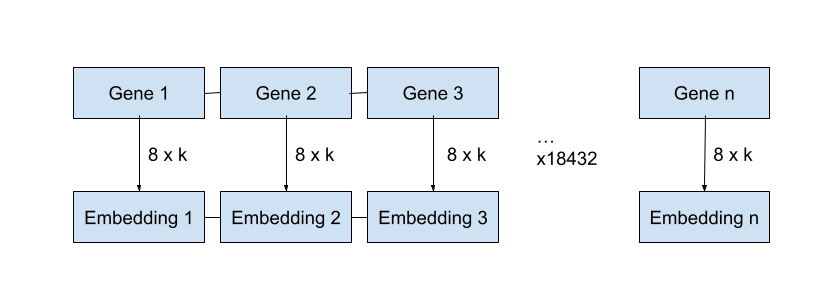
\includegraphics[width = 0.48\textwidth]{figures/MultiLayerLinear.png}
%     \caption{An overview of the proposed MultiLinearLayer}
%     \label{fig:multilinear}
% \end{figure}

\subsection{Evaluation}

The automatic evaluation of genetic diffusion models is a challenging task. Diffusion models were first pioneered in the realm of image generation, where it is comparatively easy to check if the generated data is of high quality. A human is able to inspect the generated images and can manually determine if they are realistic. 
In the genetic case this is no longer possible, as a human observer is not able to easily tell if a genetic sequence is of high fidelity. 


Furthermore, common automatic measurements from the image domain can not be applied to the genetics domain, complicating evaluation. Fréchet inception distance (FID) \citep{fid} and Inception score (IS) \citep{is} are both automatic metrics from the image domain which do not rely on a human observer and are widely regarded as good baselines for synthetic image evaluation. The problem with applying these to the genetic domain is that they rely on models which are pre-trained on large scale data to project images into a meaningful embedding space. While this kind of data is easily available in the image domain, in the genetic domain neither pre-trained models, nor the data to train them, nor data standardization are agreed upon or easy to obtain.

\subsubsection{Nearest Neighbour adversarial accuracy}
To find alternatives to these common scores we look at other scores which compare distributions.
The Nearest Neighbour adversarial accuracy is defined as \cite{yale2019privacy}:

\begin{equation} 
\begin{aligned}
        AA_{truth} = \frac{1}{n}\sum_{i=1}^n \mathbf{1} (d_{TS}(i)>d_{TT}(i)) \\
    AA_{syn} = \frac{1}{n}\sum_{i=1}^n \mathbf{1} (d_{ST}(i)>d_{SS}(i)) \\
   % AA_{TS} = \frac{1}{2}(AA_{truth}+AA_{syn}) \\
  %  PrivacyLoss = Train AA_{TS} - Test AA_{TS}
\end{aligned}
\end{equation}

Where $d(i)$ is denoting the distance of datapoint with index $i$ to the nearest neighbour, $S$ is denoting the synthetic and $T$ the real data origin. For example $d_{ST}(i)$ is the distance between the synthetic datapoint with index $i$ and the nearest neighbour from the real distribution. A score of $AA_{truth} = 0.5$ and $AA_{syn} = 0.5$ is considered optimal. 
% PrivacyLoss denotes the difference between train and test set performance. This should optimally be close to 0.
To calculate the distance to the nearest neighbour $d(i)$ we use the cosine distance metric $d_{cos}$. e.g:

\begin{equation}
    d_{cos}(x,y) = \arccos(\frac{x\cdot y}{|x|\cdot|y|}) \frac{1}{\pi}
\end{equation}

\subsubsection{Nearest Neighbour test}
The nearest neighbour (NN) test with score $S$ compares which distribution the $k$ nearest neighbours belong to.

\begin{equation}
    S(D_1,D_2) = \frac{1}{\#D_1} \sum_{D_1}^x \frac{1}{k}\sum_0^k \delta(x_{k})
\end{equation}

where $\#D$ is the number of samples in $D$ and $x_{k}$ the $k$-th nearest neighbour to $x$ in distribution $D_a = D_1 \cup D_2$, according to some distance metric, we choose the cosine distance metric. We define $\delta(x_k) = 1$ if $x_{k}\in D_1$ and 0 otherwise. An optimal score would be $S = 0.5$.

\subsubsection{UMAP}
Another common evaluation possibility is the visualization of neighbourhood structure using algorithms like UMAP \citep{UMAP} or T-SNE \citep{tsne}. Both of these methods are highly popular in the realm of Machine Learning. We choose to use UMAP due to its better performance on high dimensional data.

% \subsubsection{Linkage disequilibrium}
% Another metric which is specific to the genetic use case is Linkage disequilibrium. This metric correlates the association of alleles of different loci. By comparing the Linkage disequilibrium of our synthetic data to real data we can validate a realistic synthetic data generation.

\subsubsection{Amyotrophic Lateral Sclerosis (ALS) classification}
As the final and most important evaluation metric we use a real life binary classification task. The classification task we choose is to determine whether or not the genetic disease Amyotrophic Lateral Sclerosis is present. This task is especially suitable to evaluate if a realistic genome is produced due to its relatively high complexity, as well as the comparatively large amount of training samples which are present for this task. The task is based on 10.405 examples which were diagnosed by medical professionals into 3192 ALS positive and 7213 negative samples. The task does not exhibit simple reliance on one or even multiple genomes and at least 1000 genomes are needed to obtain good performance \citep{capsulenet}.  

We train a simple classifiers to perform binary classification. If the classifier can also be trained on synthetic data and still performs well on a holdout test set of real data we can conclude that the features used for ALS classification were well reproduced.
To ablate against the type of classifier having a large impact we evaluate using 3 different classifiers: MLP, Transformer and CNN.
% \begin{itemize}
%     \item MLP
%     \item Transformer
%     \item CNN
% \end{itemize}

All evaluations will be performed on a balanced hold out test set of 520 positive and 520 negative examples for a total of 1040 samples or 10\% of the total available data. We follow the experimental protocol of \citet{capsulenet} to achieve easy to compare results.

\section{Experiments}
\label{sec:experiments}

In this section we will look at the results of the models proposed in Section \ref{sec:methods}. 


\subsection{Training Metrics}
First we show loss curves during training on train and validation data of the different diffusion model types, see Figure \ref{fig:losscurvesall}.



We observe that no models have any problems with over-fitting. The CNN based models overall performs best with regards towards minimizing the train loss.

% \begin{figure}[t]
%     \centering
%     \subfloat[train]{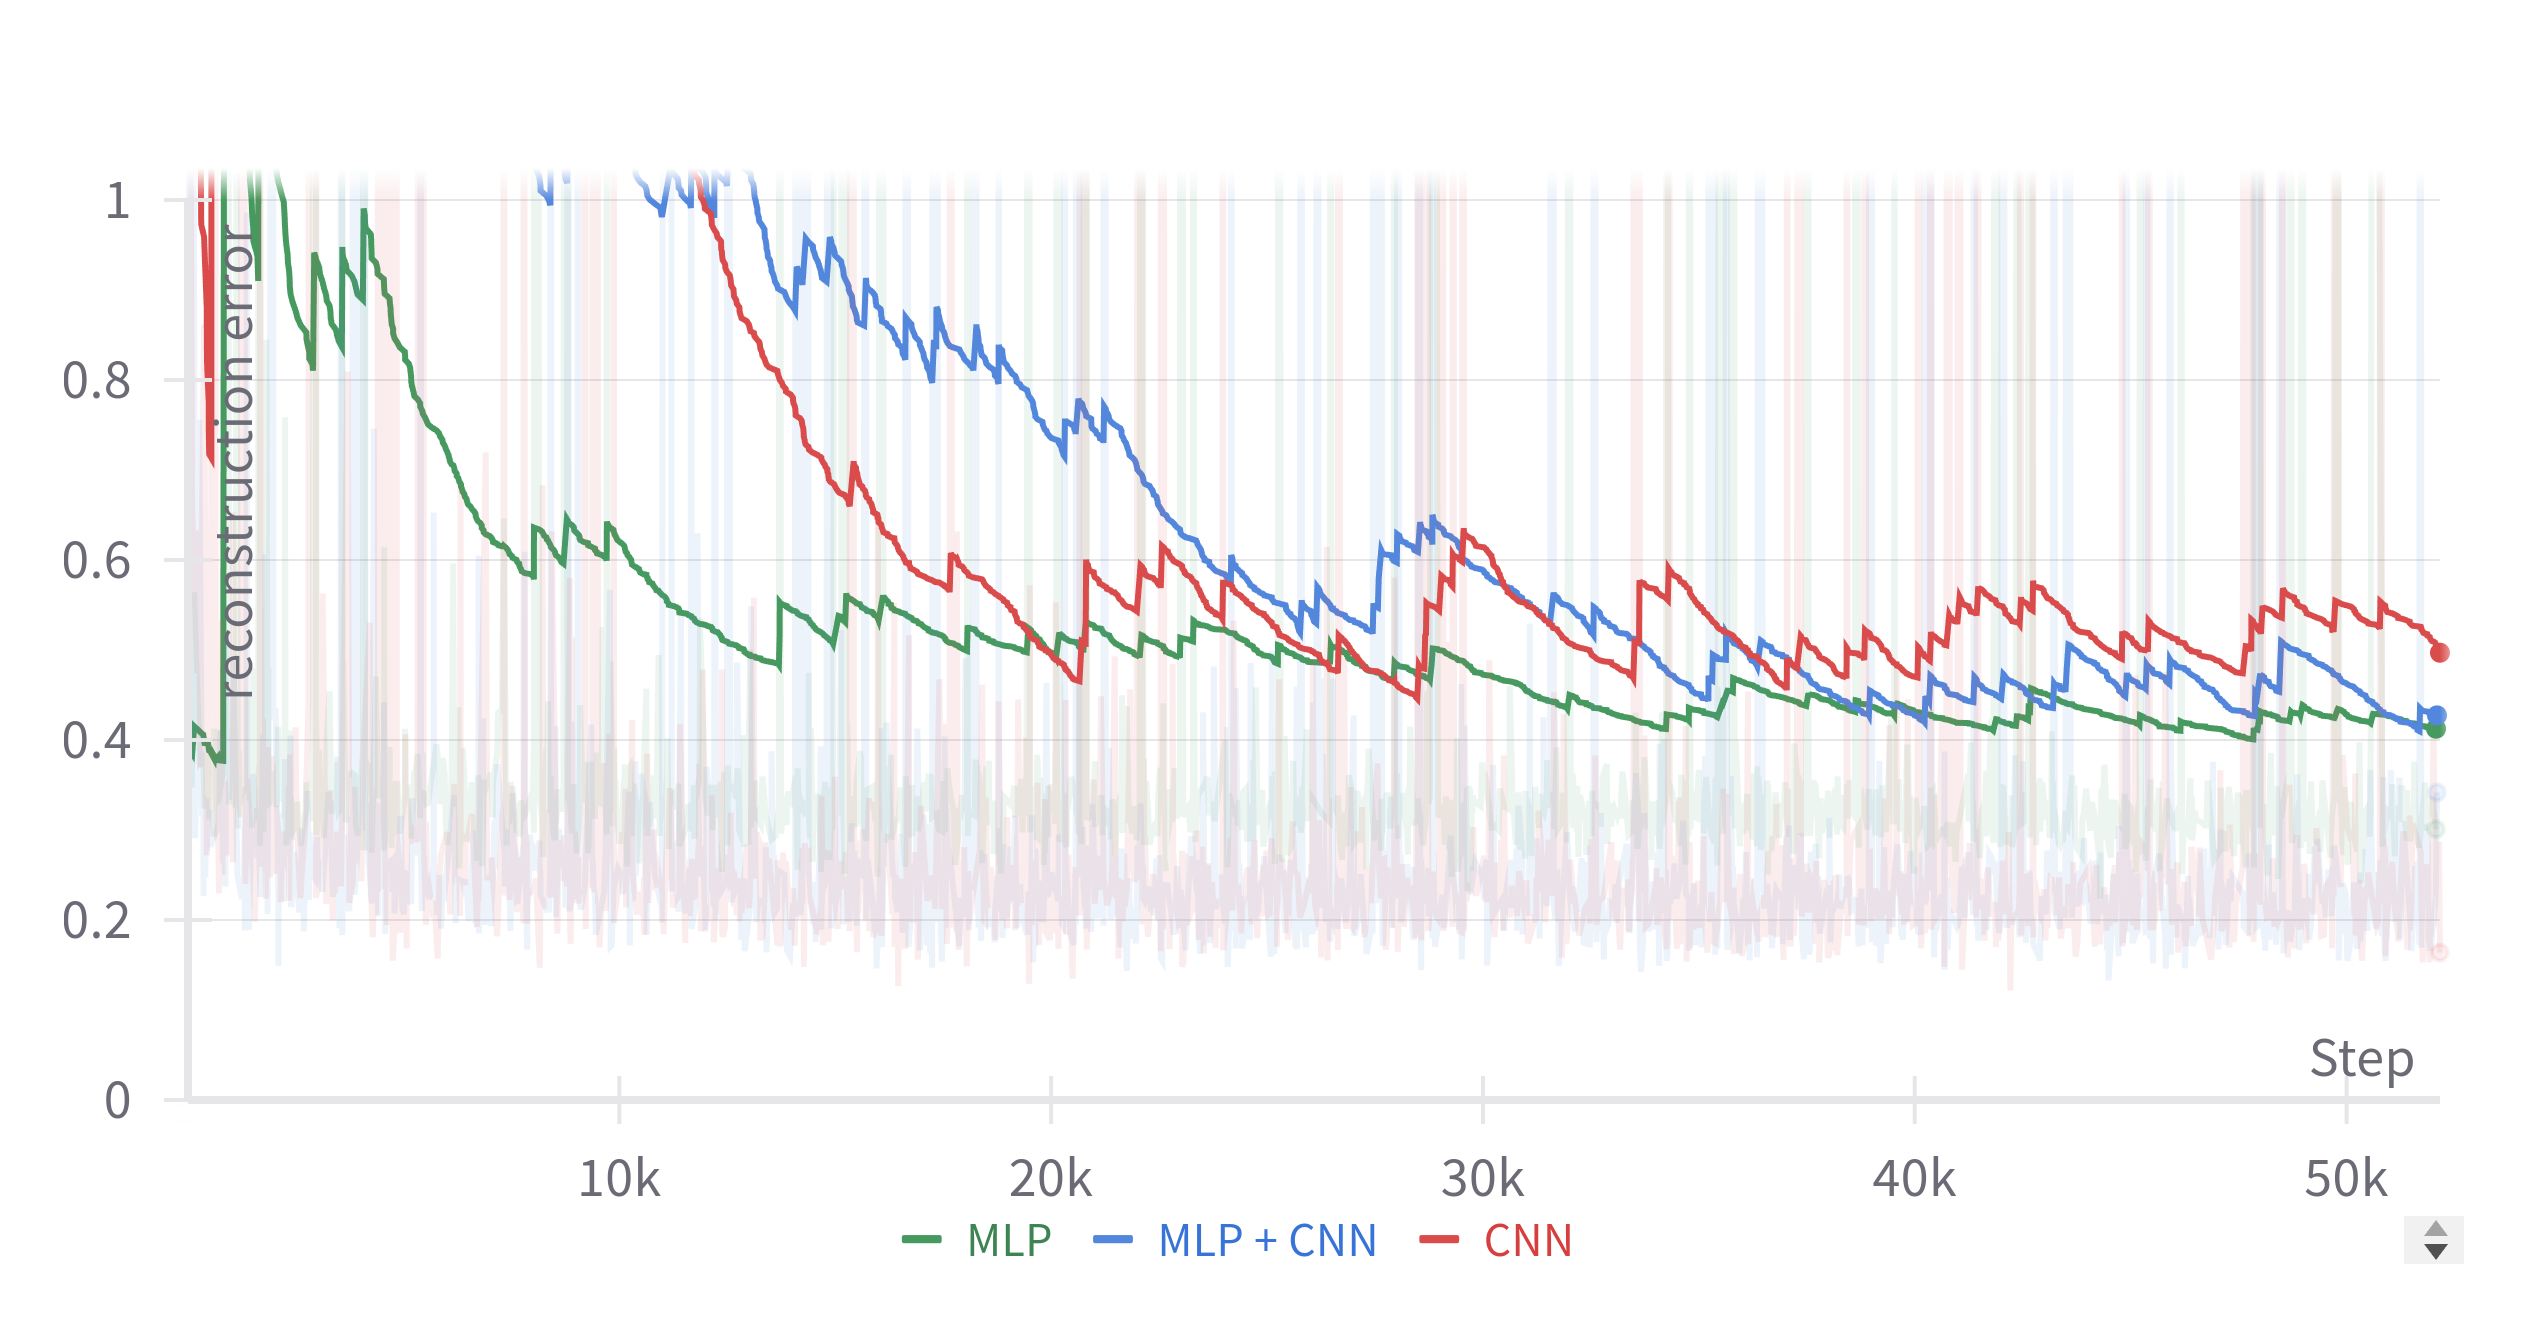
\includegraphics[width = 0.33\textwidth]{figures/reconstruction_error.png}}
%     \subfloat[validation]{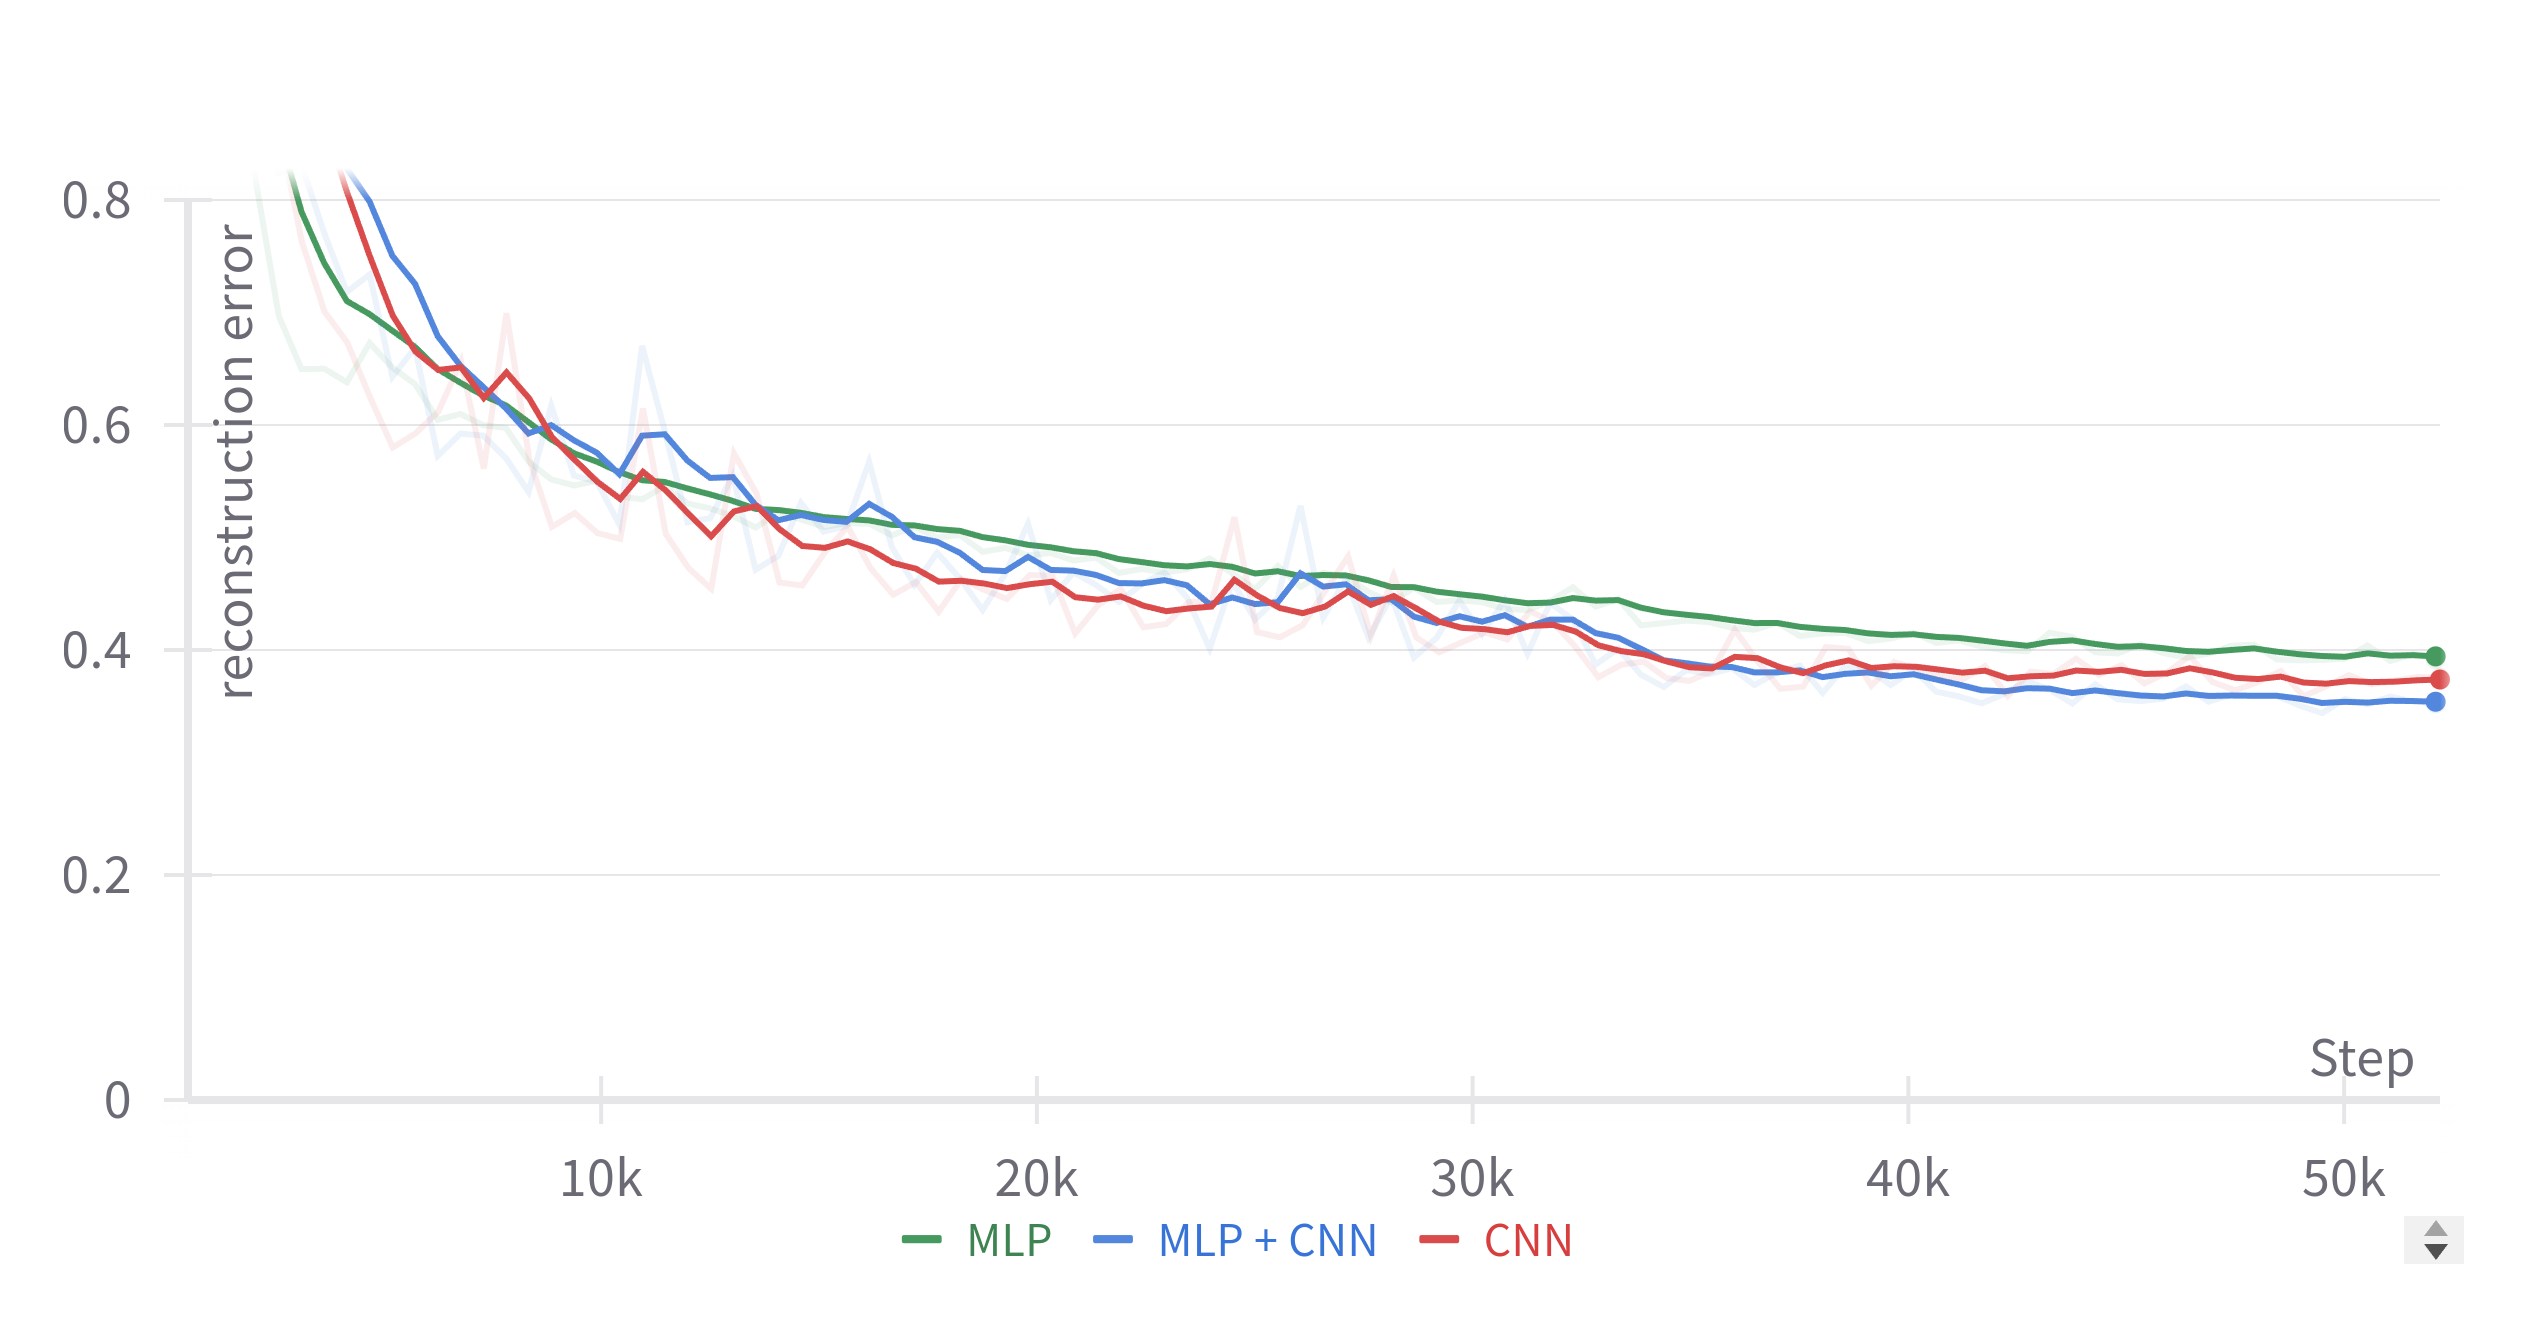
\includegraphics[width = 0.33\textwidth]{figures/valrecerror (1).png}}  

%     \caption{}
%     \label{fig:recerror}
% \end{figure}



However, if we take a closer look at the reconstruction error of the model, visualized in Figure \ref{fig:losscurvesall}, we note that the MLP model actually performs surprisingly similar to the CNN model and that even though only very small drops in loss during training can be observed for the MLP, the reconstruction error keeps improving. The Transformer based architecture seems to be performing decently in loss and reconstruction error.
We note that reconstruction error is highly related to the loss, but scaled by the noise schedule $t$, e.g. this error focuses more on large values of $t$.

To further analyze this, in Figure \ref{fig:lossvsnoise} we visualize the reconstruction error curves vs amount of noise added of the different diffusion models. We can see that while the CNN has an overall better performance it focuses more on the fine detail of the structure e.g. recovering from small noise values, while the MLP architecture is more focused on recovering rough structure (e.g. high noise). 
\begin{wrapfigure}{r}{0.5\textwidth}
  \centering
  \subfloat[train loss]{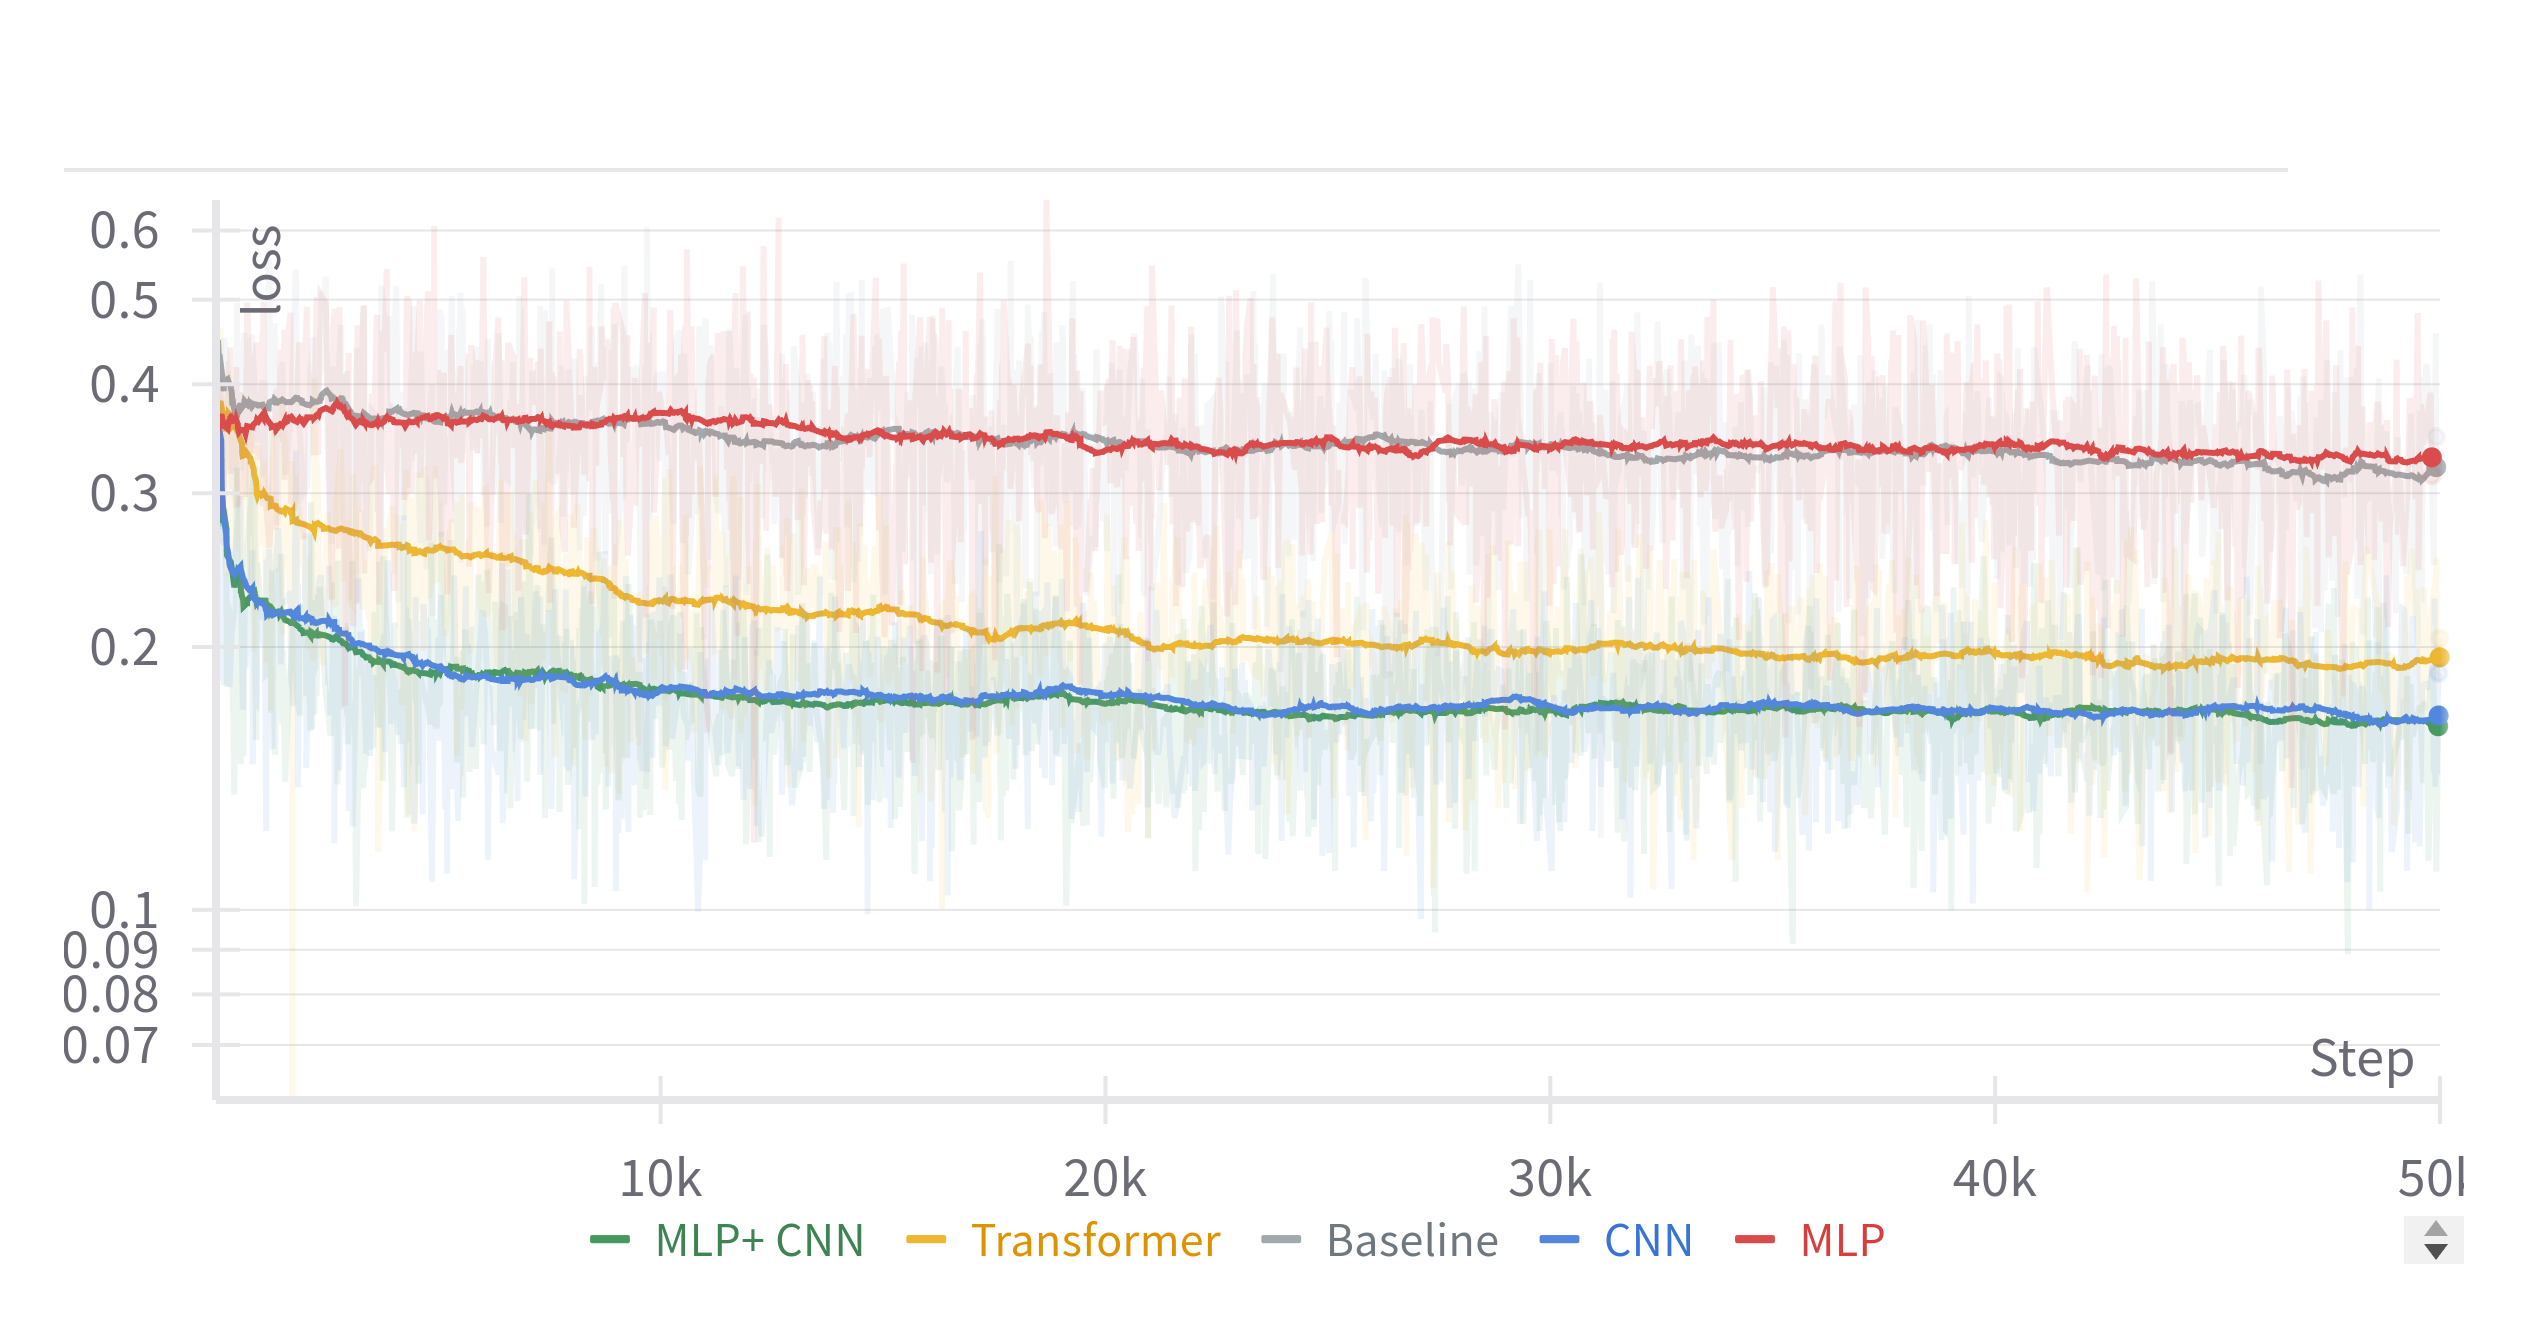
\includegraphics[width = 0.25\textwidth]{figures/losstrain.png}}
  \subfloat[validation loss]{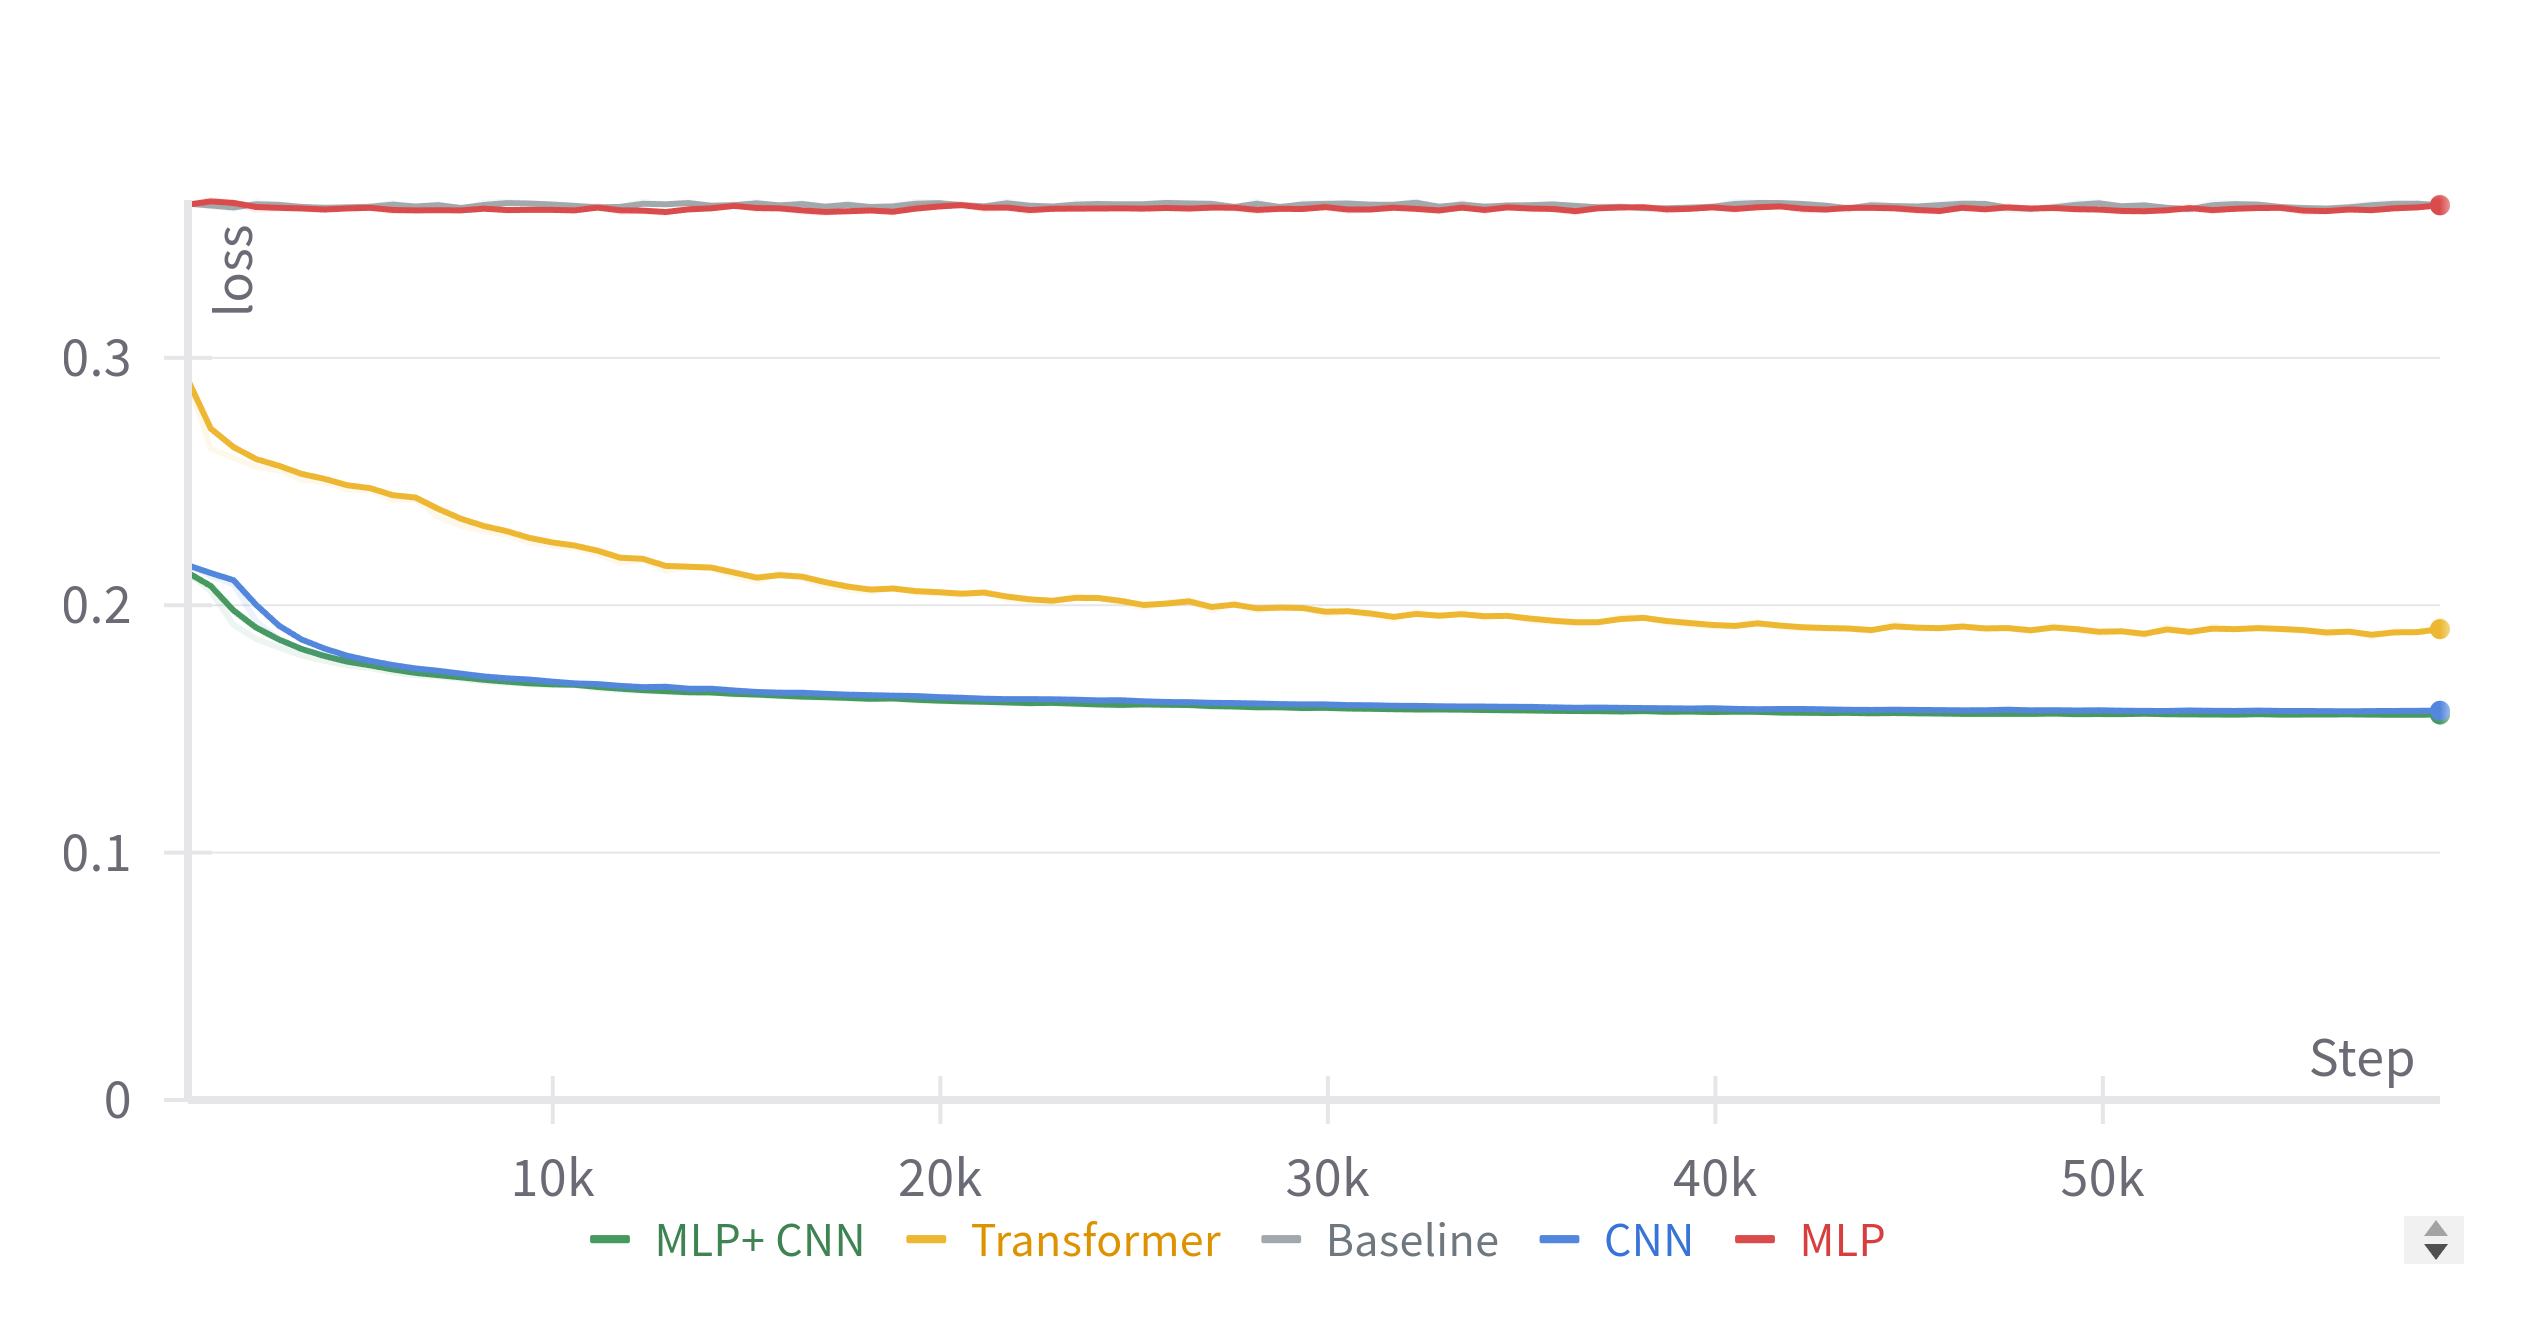
\includegraphics[width = 0.25\textwidth]{figures/lossval.png}}   \\

  \subfloat[train rec error]{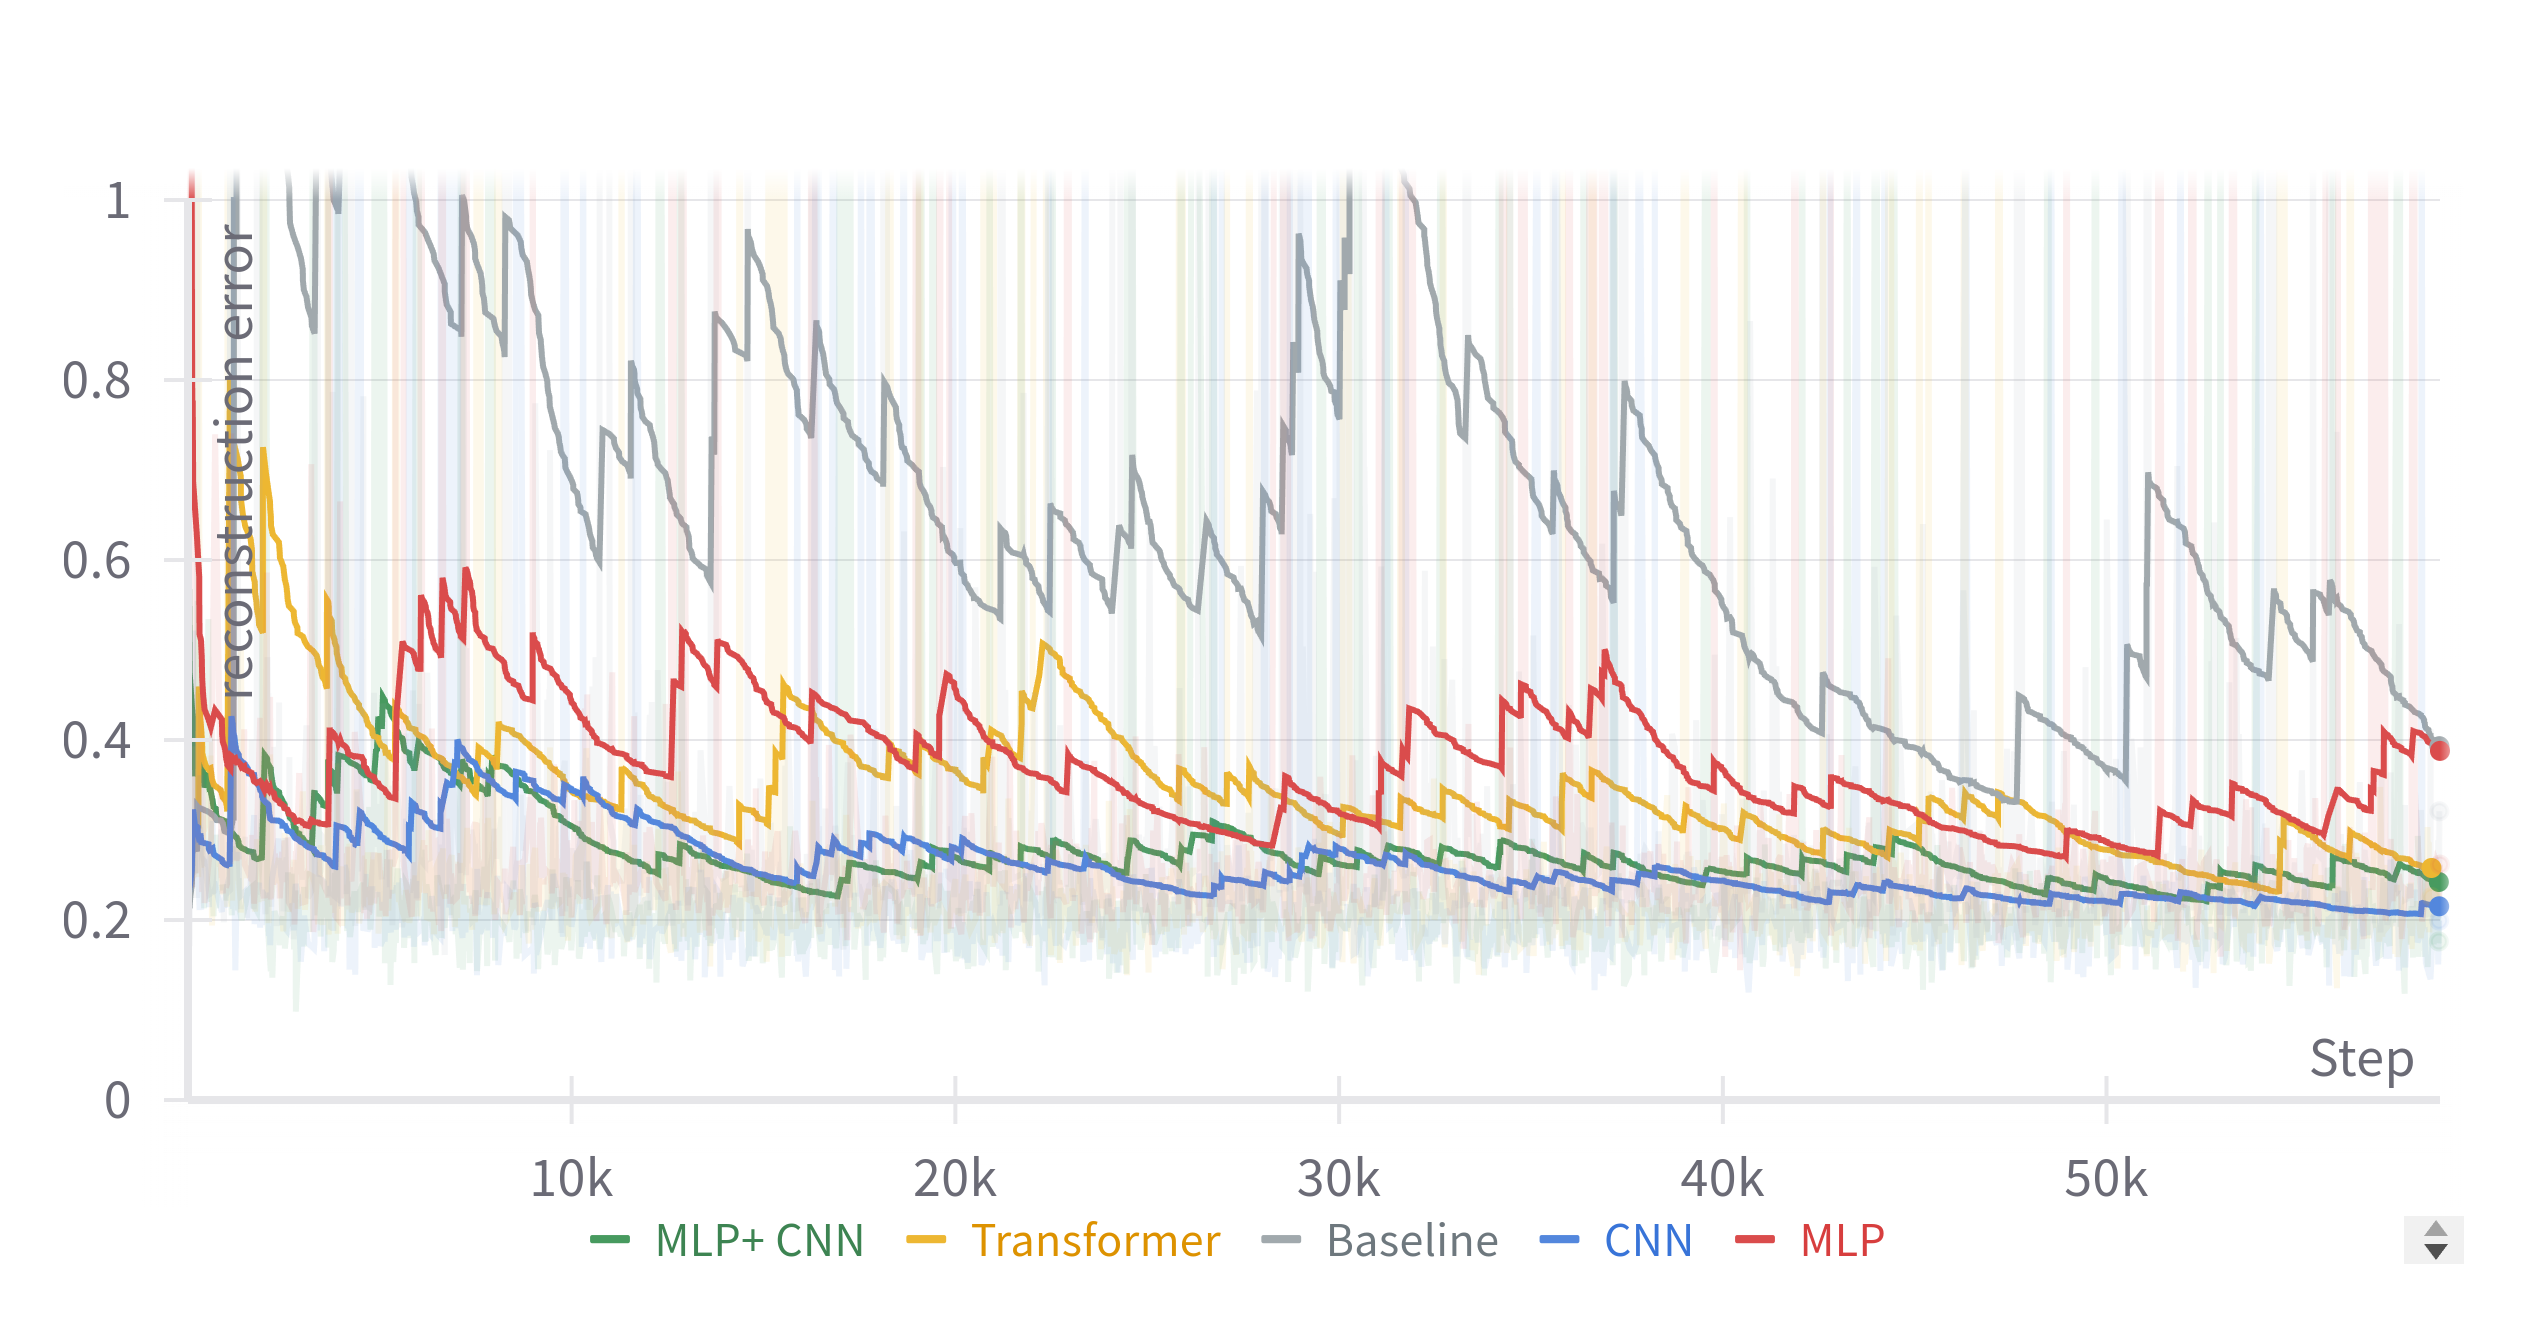
\includegraphics[width = 0.25\textwidth]{figures/recerrortrain.png}}
  \subfloat[validation rec error]{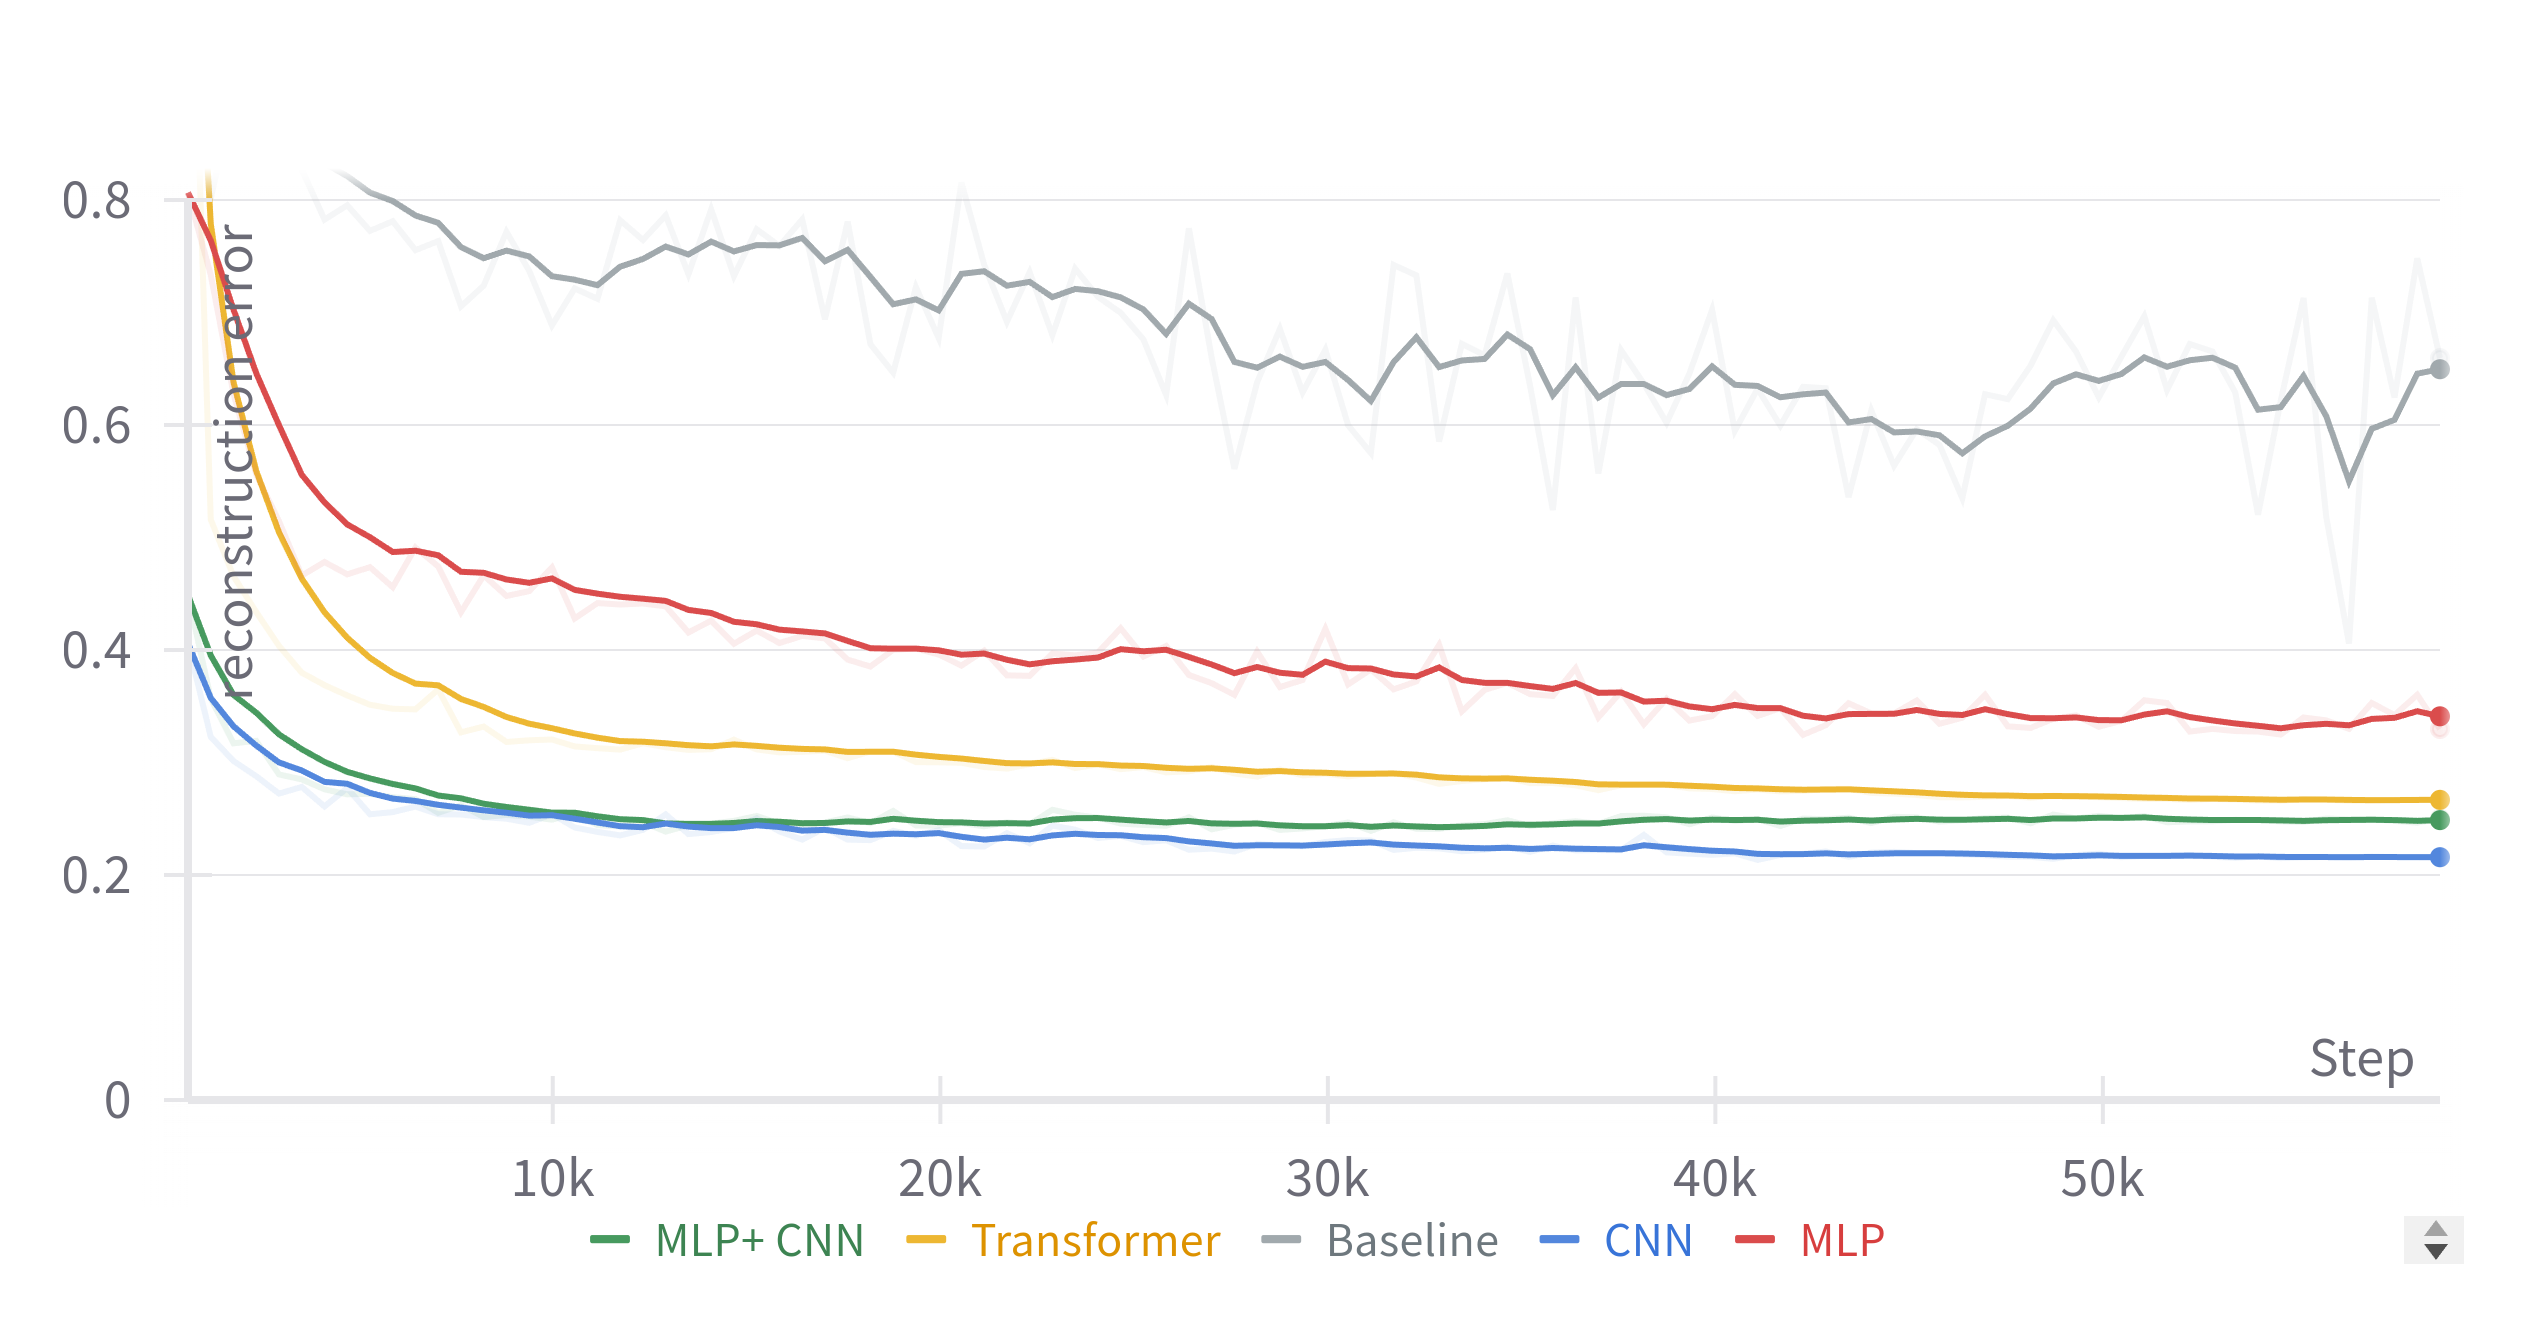
\includegraphics[width = 0.25\textwidth]{figures/recerrorval.png}}

  \caption{Top curves are smoothed loss curves for all diffusion model architectures during training on train and validation data. Bottom curves are smoothed reconstruction error e.g. $||x_p,x||$ during training and validation using single shot denoising according to Eq \ref{eq:denoise}.}
  \label{fig:losscurvesall}
\end{wrapfigure}

\begin{figure}
    \centering
    \subfloat[CNN]{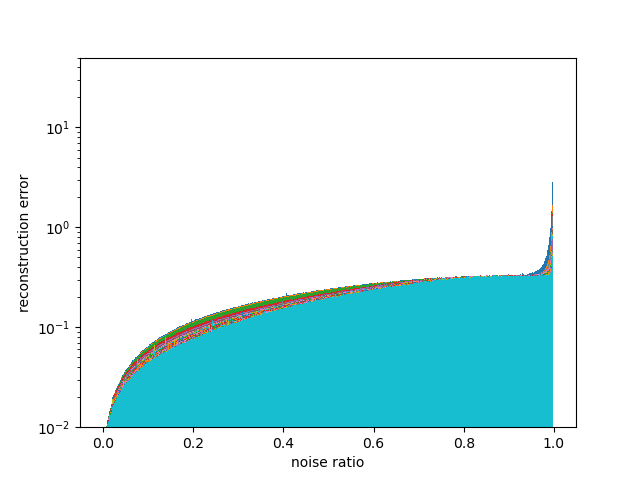
\includegraphics[width = 0.33\textwidth]{figures/Cnn.png}}
    \subfloat[Transformer]{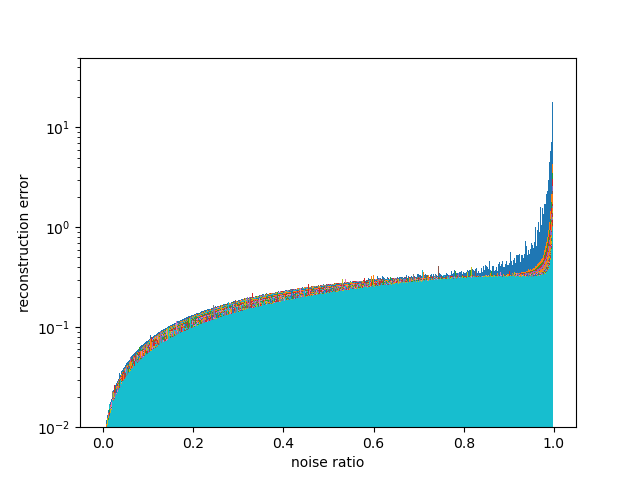
\includegraphics[width = 0.33\textwidth]{figures/Transformer.png}}  
    \subfloat[MLP]{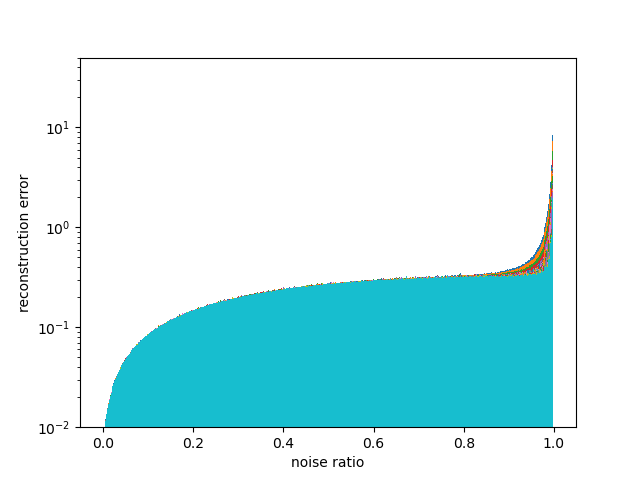
\includegraphics[width = 0.33\textwidth]{figures/MLP.png}}  

    
    \caption{Reconstruction error vs noise curves during training for different diffusion model backbones. Note the logarithmic scaling of the y-axis. }
    \label{fig:lossvsnoise}
\end{figure}



\subsection{Evaluation}

\begin{wrapfigure}{r}{0.5\textwidth}
  \centering
  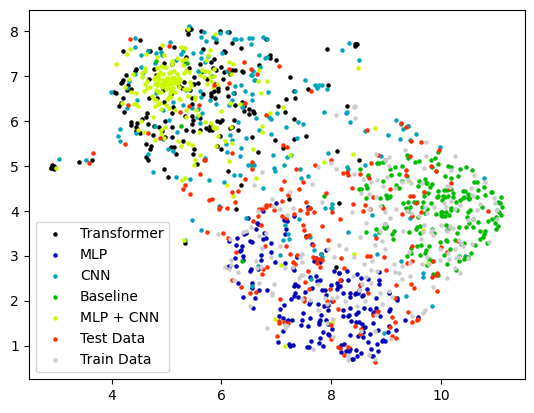
\includegraphics[width = 0.48\textwidth]{figures/umap.png}
  \caption{UMAP visualizations of data of different origins. Red and grey points are test and train data (real). Blue is MLP, green is Baseline. Yellow, black and bright blue are MLP + CNN, Transformer and CNN respectively.}
  \label{fig:umap}
\end{wrapfigure}
Next we take a closer look at the performance of a classifier trained on synthetic vs real data, see Table \ref{Fig:cls}. We observe the MLP generated data performing superior compared to all other synthetic data types with around $84.7\%$ accuracy, whereas the CNN based data fails to capture the relations important for ALS classification with the best performance of $62.64\%$ and the Transformer generated data having a maximum accuracy of $64.62\%$ on the real test data.
Training on real data is performing best with $87.6\%$ accuracy, as expected.

% \begin{figure}[t]
%     \centering
%     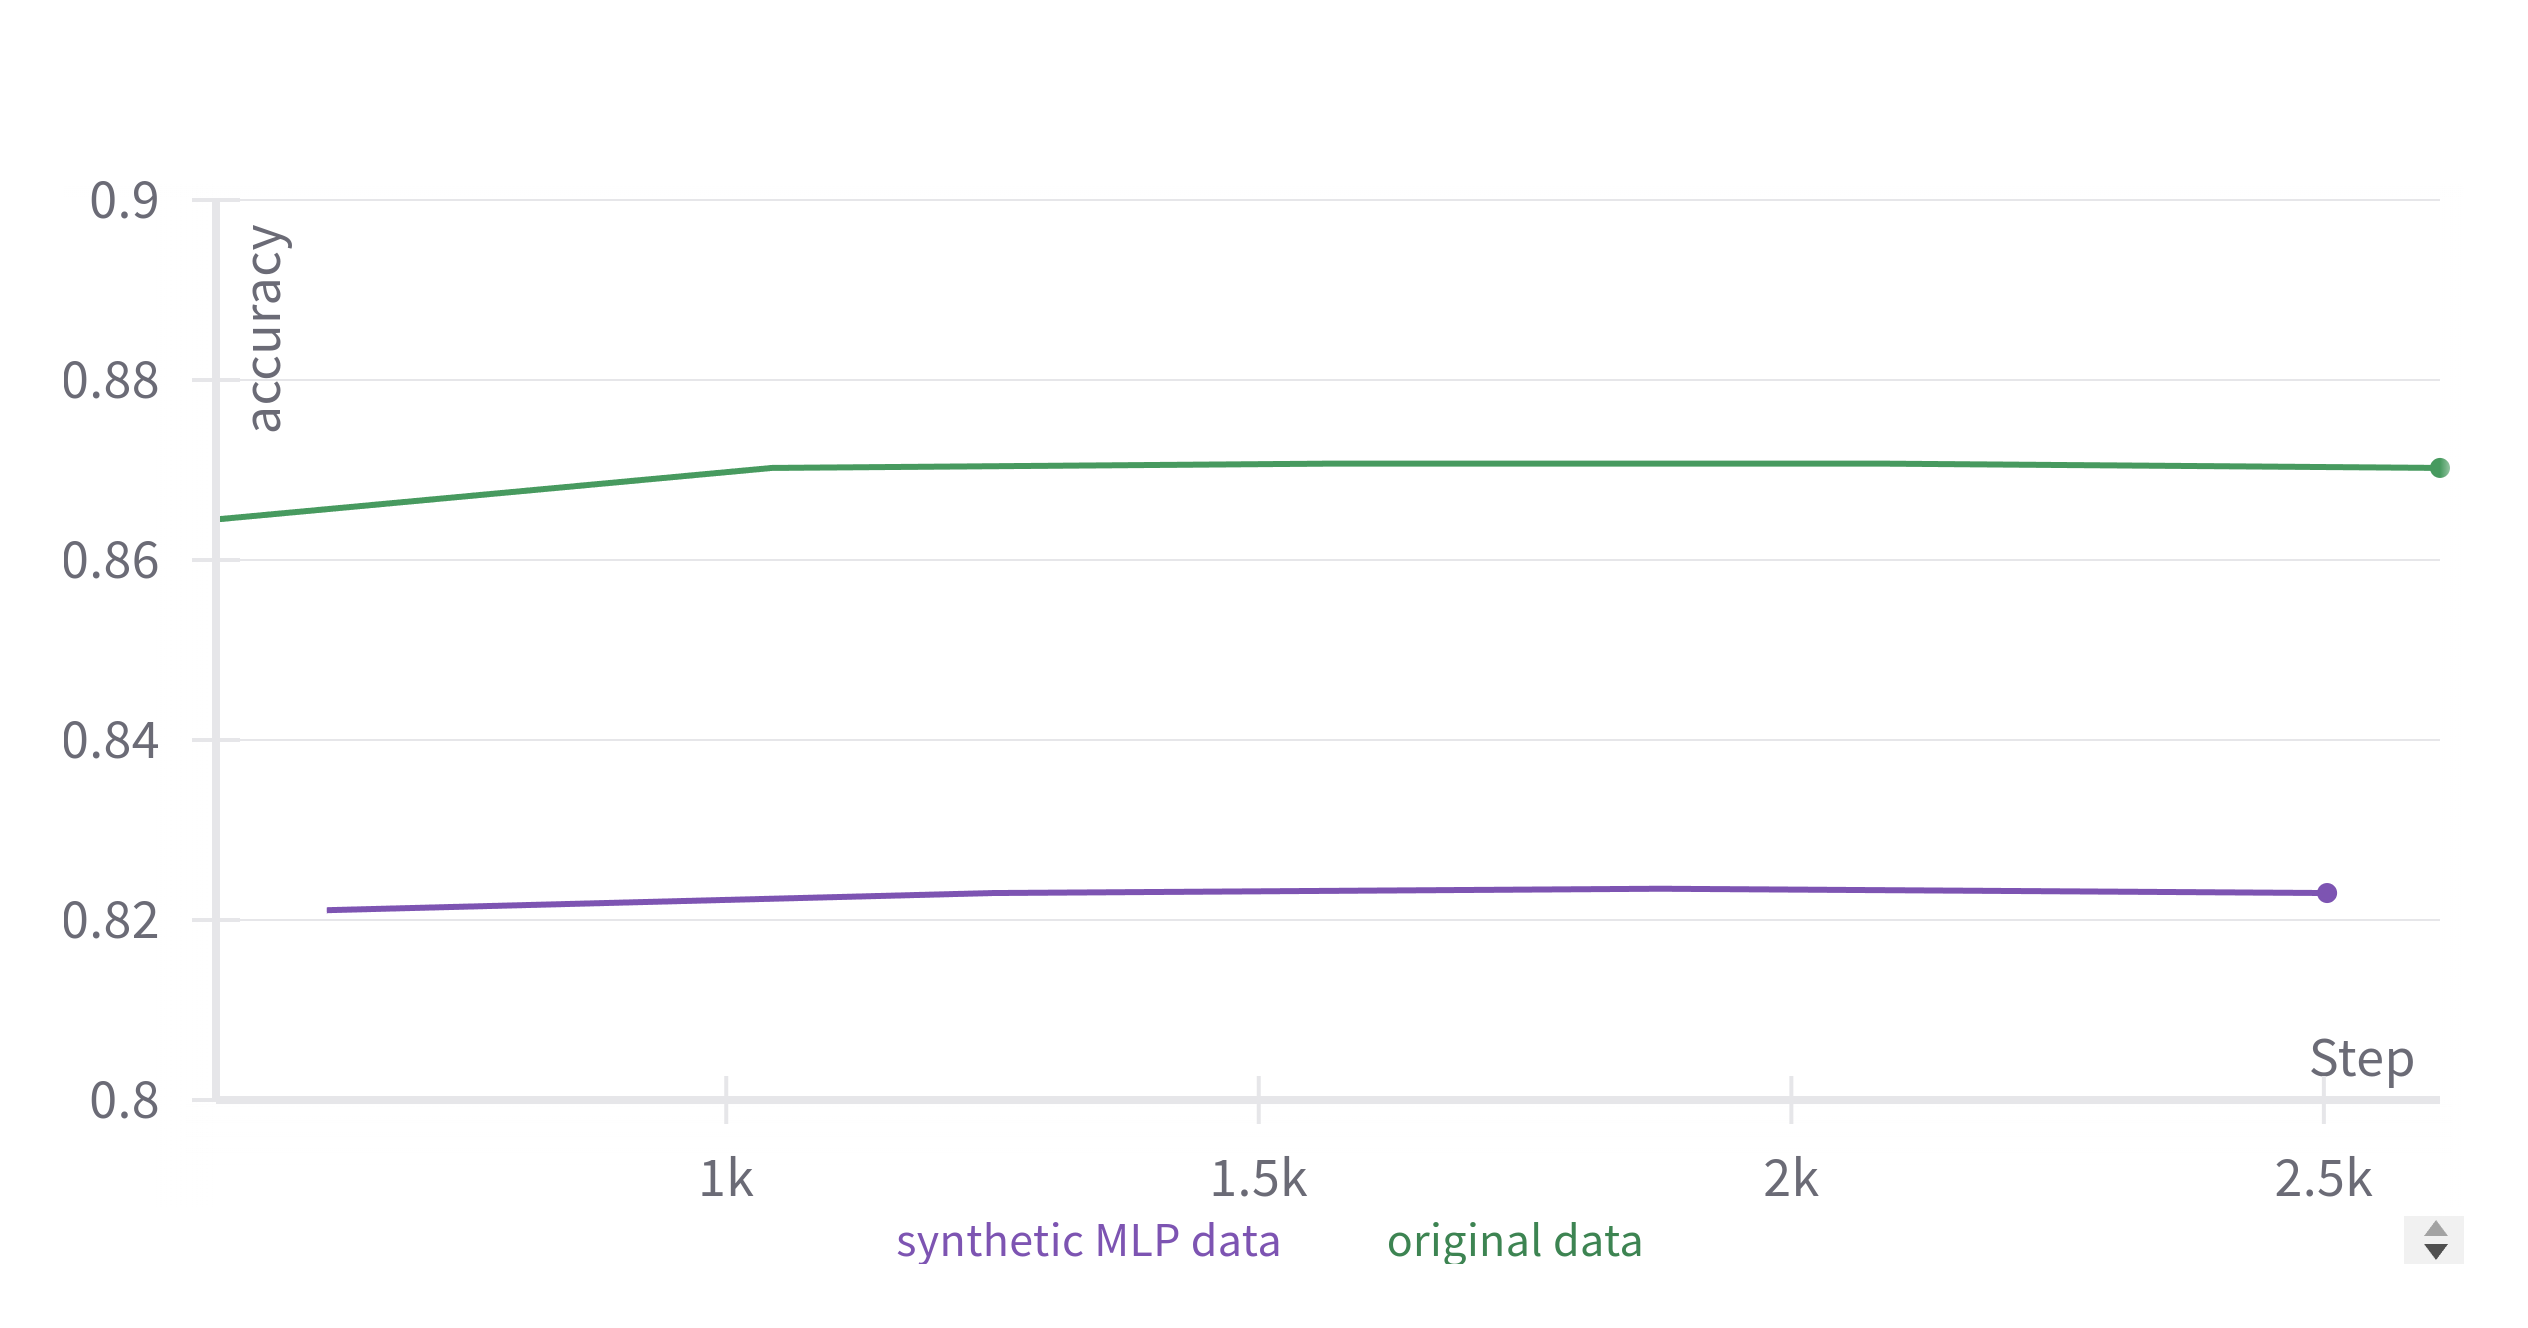
\includegraphics[width = 0.48\textwidth]{figures/test_acc.png}
%     \caption{Test accuracy on MLP generated and Baseline data. CNN generated data not visualized due to poor performance.}
%     \label{fig:cls}
% \end{figure}

\begin{table}
  \centering
  \caption{Accuracy on a hold out test set after training different ALS classifier (MLP, Transformer or CNN)  on different synthetically generated data types (generated by: MLP, Transformer, CNN, MLP + CNN or Baseline). The best synthetic data for each classifier type is marked in \textbf{bold}.}
  \label{Fig:cls}
  \begin{tabular}{c|cccccc}
    \toprule
Classifier & Real Data  & CNN  & MLP  & MLP + CNN & Transformer & Baseline \\
 
   \cmidrule(r){1-7} 
MLP &  87.60 & 62.64 & \textbf{84.71} & 82.21 & 64.62 & 70.19 \\
Transformer & 82.11  & 54.23 &  \textbf{76.73} & 71.06 & 56.92 & 45.10 \\
CNN &  73.17 & 51.15 & \textbf{67.11} & 50.00 & 50.29 & 50.00 \\
\cmidrule(r){1-7} 
average & 80.79 & 56.01 & \textbf{76.18} & 66.01 & 57.28 & 55.10\\
    \bottomrule
  \end{tabular}
\end{table}



% In Table \ref{Fig:nndistance}, we show the results of the nearest neighbour score. One possibility for the diffusion model to produce convincing results is by reproducing the data it was trained on. To rule out this possibility we take a closer look at the nearest neighbour score. We compute this score from the original training distribution $D$ to itself as a Baseline and to the data generated by the MLP and the CNN model. We observe that while the CNN has a lower distance than the baseline, which indicates some possibility of reproduction, our more successful MLP model actually has a very high score, which indicates a very diverse set of newly generated data points.

% \begin{table}
%   \centering
%   \caption{Result of nearest neighbour score for datasets generated by the MLP as well as the CNN models as well as a baseline.}
%   \label{Fig:nndistance}
%   \begin{tabular}{ cccc}
%     \toprule
% Baseline  & CNN & MLP & Transformer  \\
 
%   \cmidrule(r){1-4} 
%  63293 & 79168 & 70261 &  \\


%     \bottomrule
%   \end{tabular}
% \end{table}

% \begin{table}
%   \centering
%   \caption{Result of Nearest Neighbour adversarial accuracy for datasets generated by the MLP as well as the CNN models as well as a baseline.}
%   \label{Fig:nndistance}
%   \begin{tabular}{c cc}
%     \toprule
%   & CNN & MLP  \\

%   \cmidrule(r){1-1}  \cmidrule(r){2-3} 
%    $AA_{truth}$ & 0.4 & 0.55 \\
%    $AA_{syn}$& 0.0 & 0.18  \\
%    $AA_{TS}$ & 0.2 & 0.365 \\
%  Privacy Loss & -0.07 & 0.015 \\


%     \bottomrule
%   \end{tabular}
% \end{table}




In Figure \ref{fig:umap}, we visualize the distribution of different data types using UMAP \citep{UMAP} with cosine distance metrics. Euclidean distance metrics are notoriously bad for high dimensional data and return uniform distributions.
%Red and grey points are real test and train data. Blue data points are generated by MLP, green ones by Baseline. Yellow, black and bright blue ones are generated by MLP + CNN, Transformer and CNN respectively.
We observe that the UnetMLP generated data is closest to the real data in the UMAP visualization. 
The Baseline generated data is close to some of the training data (grey) but comparatively little of the test data (red), indicating over-fitting on the training set, this is especially interesting as Figure \ref{fig:losscurvesall} does not indicate any over-fitting during training.
The Transformer, CNN and MLP + CNN generated points are all clustering together with only small overlap with the training or test data.
Even though this UMAP visualization can give us an indication of neighbourhood structure, we want to emphasize that the visualizations can be highly misleading. In this example, MLP + CNN and CNN generated points are similarly visualized while the classification task performance, see Table \ref{Fig:cls}, is very different in between both groups. 
%Real Training data is red, validation data is brown, CNN generated data is blue and MLP generated data is green. No clear clusters seem to be forming, neither according to the baseline classes of ALS positive/negative or due to the origin of the data. Thereby we conclude that either UMAP is not able to discern complex relationships and/or the generated data is of sufficient quality to be similar enough.



Next we look at the nearest neighbour test and the nearest neighbour adversarial accuracy, see Tables \ref{Fig:nnacc} and \ref{Fig:nntest}. We observe MLP+CNN performing best for the nearest neighbour test and CNN performing best for nearest neighbour adversarial accuracy. While these test shed some light on the quality of the generated data, we do not think that distance metrics on the high dimensional input data are especially meaningful. This strongly reduces the value of these tests.


\begin{table}
  \centering
  \caption{Result of nearest neighbour test (k=10) for all datasets. Closer to 0.5 is better. Best performance is marked in \textbf{bold}.}
  \label{Fig:nntest}
  \begin{tabular}{c|ccccc}
    \toprule
comparison data &  CNN & MLP & MLP + CNN &Transformer & Baseline \\
   \cmidrule(r){1-6} 
train & 0.7835 & 0.0165 & \textbf{0.4039} & 0.7935 & 0.0265  \\
test &  0.7755 & 0.2825 & \textbf{0.3740} & 0.765 & 0.3515 \\


    \bottomrule
  \end{tabular}
\end{table}

\begin{table}
  \centering
  \caption{Result of Nearest Neighbour adversarial accuracy for generated datasets. Closer to 0.5 is better. Best performance is marked in \textbf{bold}.}
  \label{Fig:nnacc}
  \begin{tabular}{c ccccc}
    \toprule
  & CNN & MLP  & MLP + CNN & Transformer & Baseline \\

  \cmidrule(r){1-1}  \cmidrule(r){2-6} 
   $AA_{truth}$ & 0.755 & 0.225  & \textbf{0.415} & 0.915 & 0.35\\
   $AA_{syn}$& \textbf{0.62} & 1.0  & 0.925 &  0.65 & 0.995 \\
  % $AA_{TS}$ & 0.6875 & 0.6125  & 0.67 &  0.7825 & 0.6725 \\
% Privacy Loss & -0.07 & 0.015 \\


    \bottomrule
  \end{tabular}
\end{table}

\section{Conclusion}

In this work we presented the first full human genome diffusion models.
By creating synthetic human genomes we are able to address the problem of sharing highly sensitive data by replacing it with non sensitive synthetic data. We show that the synthetic data quality is sufficient to train on and achieve good results for ALS classification, as well as use a variety of other metrics to evaluate the quality of the generated data.

Further work is needed to extend this proof of concept to real world applications. The first step could be to improve the generated genomes, either by increasing the available training data for training the diffusion model or improving the diffusion model architecture. 

We look forward to the input of the scientific community and potential applications.

We publish all code at [anonymized for review].

\bibliographystyle{plainnat}
\bibliography{reference}

\end{document}